\section{Stardice response}
\label{sec:rsd}

In this section, we will show the methodology to obtain the \SD telescope response $\Rtel$ from the Equation~\ref{eq:rsd}.

\subsection{Data set description}
\label{sec:sd_datadesc}

As described in section \ref{sec:cbp_datadesc}, the laser emits pulses at a rate of \SI{1}{\kilo\hertz} in bursts that are separated with dark times. Figure~\ref{fig:ccd_examples} shows examples of images obtained when the CBP shoots in the \SD CCD camera with two different pinholes. 

\begin{figure}[h]
    \centering
    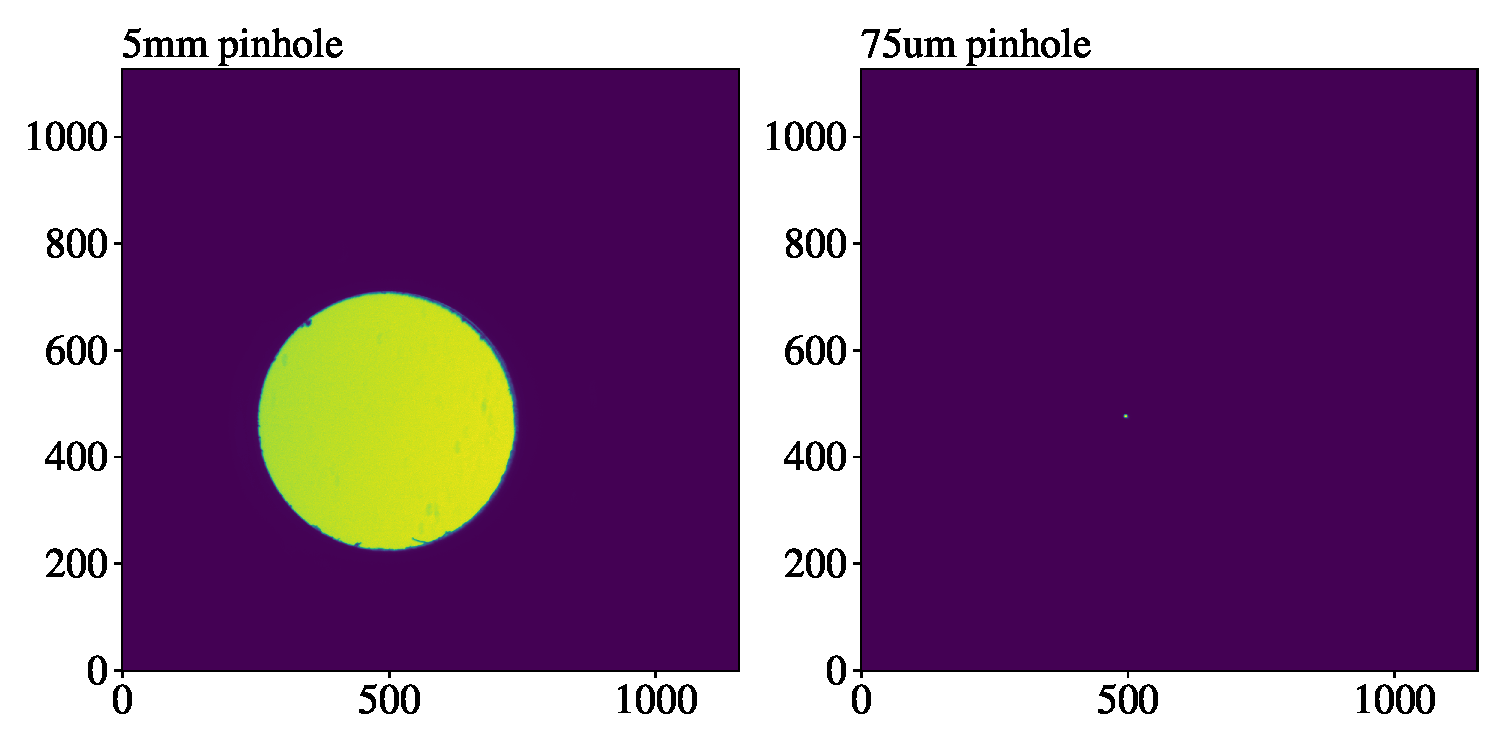
\includegraphics[width=\columnwidth]{fig/ccd_examples.pdf}
    \caption{Examples of images obtained when the CBP shoots in the \SD telescope with the CBP at \lambda_L=\SI{450}{\nm}, with the \bpinhole on the left and \spinhole on the right.}
    \label{fig:ccd_examples}
    %/stardice/analysis/cbp_paper/golden_sample_analysis/dr2/npulses_stardice.ipynb
\end{figure}

%The number of pulses per burst is tune to maintain a roughly constant cumulated charge in the photodiode at every wavelength to avoid a non-linearity behaviour. It is also constrained by the saturation limit of the CCD camera. 
%
% We had to deal with the saturation of the CCD camera and we show in the Figure~\ref{fig:saturation_lim} the maximal value in the CCD camera for one pulse. The CCD camera being highly sensitive, two pulses can be enough to saturated the pixels enlightened at some wavelengths. Our capacity to have a constant cumulated charge in the CCD camera is then limited by the finite value of pulses that we can send. 
% 
% The pinhole diameter, the point of impact on the \SD primary mirror, the point of incidence on the \SD focal plane and the bands studied can vary from a measurement to another. All these informations can be found in table \ref{tab:schedule}.
%
%\begin{figure}[h]
%    \centering
%    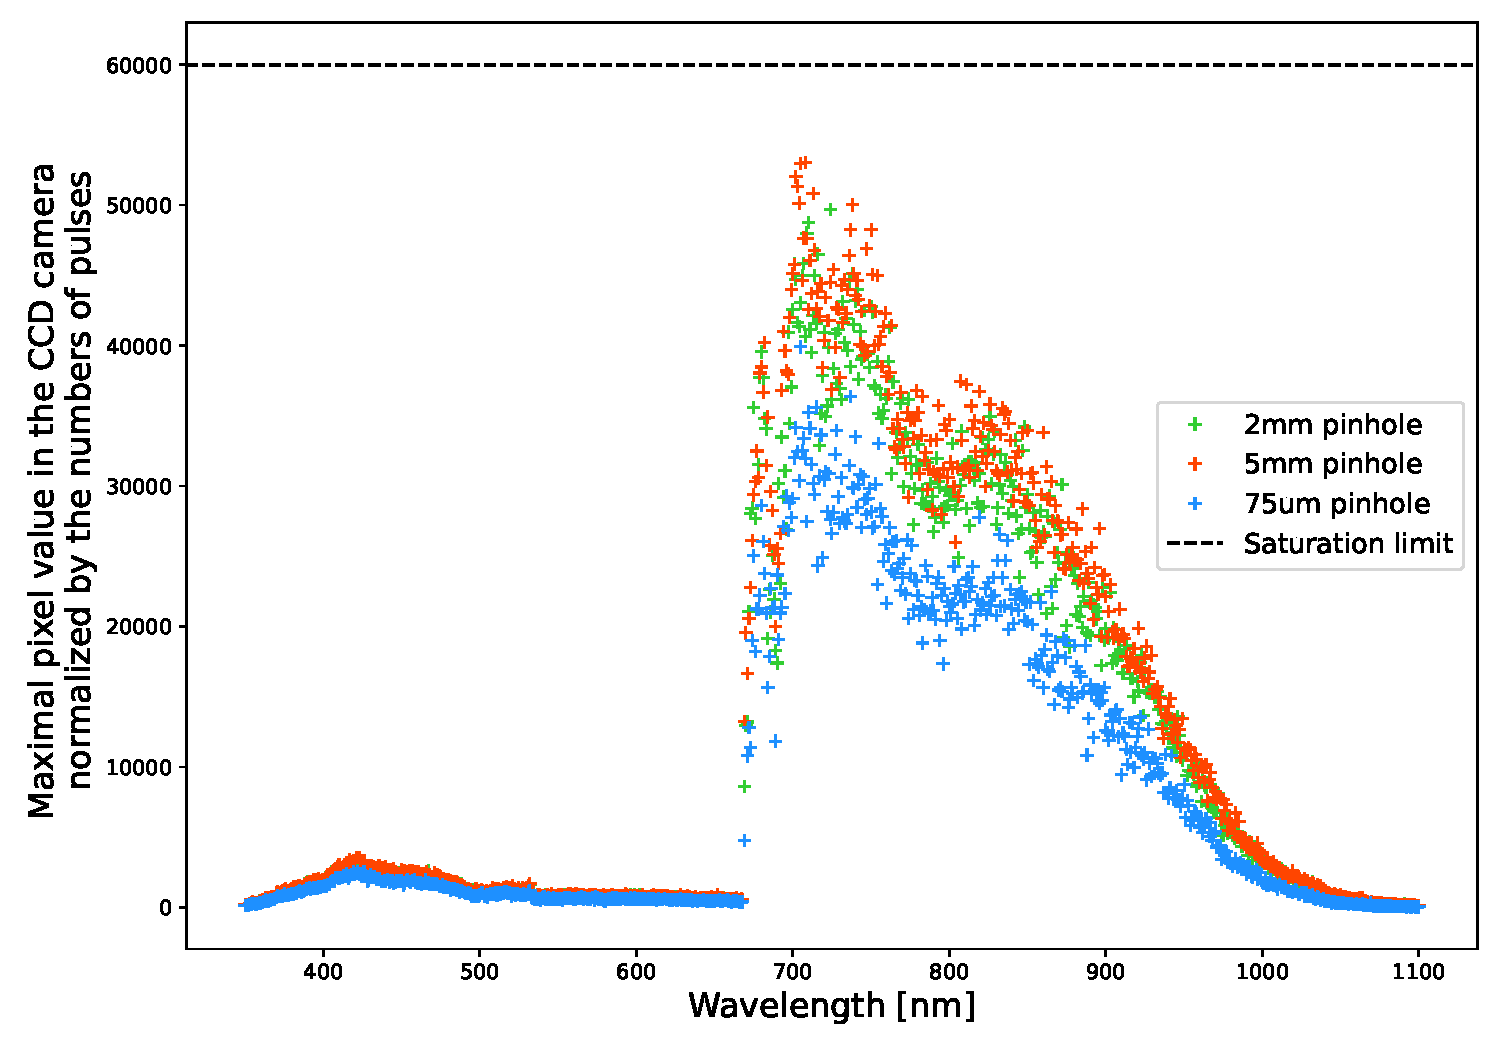
\includegraphics[width=\columnwidth]{fig/saturation_lim_ccd.pdf}
%    \caption{Maximal pixel value in ADU measured in the CCD camera of \SD normalized by the number of pulses and the saturation limit of the camera estimated at \SI{61600}{ADU}, against the wavelength. Here we can see that for some wavelengths above \SI{668}{\nano\meter} a few number of pulses can saturate the camera.}
%    \label{fig:saturation_lim}
%    %/stardice/analysis/cbp_paper/golden_sample_analysis/dr2/npulses_stardice.ipynb
%\end{figure}

\subsection{Reduction of images}
\label{sec:photometry}

Data reduction for the monitoring photodiode and the spectrograph are the same as described respectively in the section \ref{sec:pd_reduction} and \ref{sec:spectro_reduction}. Firstly, we want to estimate subtract the overscan in every image. We compute the mean of the vertical overscan of each column, and the mean of the horizontal overscan of each row. For each pixel $(i, j)$, we subtract the sum of estimation of the overscan estimated on the column $i$ and the row $j$.
Then, aperture photometry is done to extract the cumulated charge from the \SD camera images.  This requires a background subtraction, and two differents methods are used depending on the pinhole.

\subsubsection{\spinhole pinhole}

To estimate the background contribution, it is necessary to detect the sources in the image and mask them. We compute the standard deviation of an image $\sigma$, and every pixel with a signal higher than 5$\sigma$ is masked, as well as all the surrounding pixels that has a signal higher than 2$\sigma$. Then we proceed to a segmentation of the masked image into boxes of $129\times132$ pixels. We compute the mean and the standard deviation of the background in each of these boxes, and we interpolate their values in a 2D map to get our estimation of the background. This background is subtracted to the image, then we compute the centroid of the spot of interest. We measure the number of charges $\Qccd$ with aperture photometry at a radius of 21.2 pixels on this image without background. With this method, we are able to extract the charges $\Qccd$ for every image of the dataset with the \spinhole.

%\begin{figure}[h]
%    \centering
%    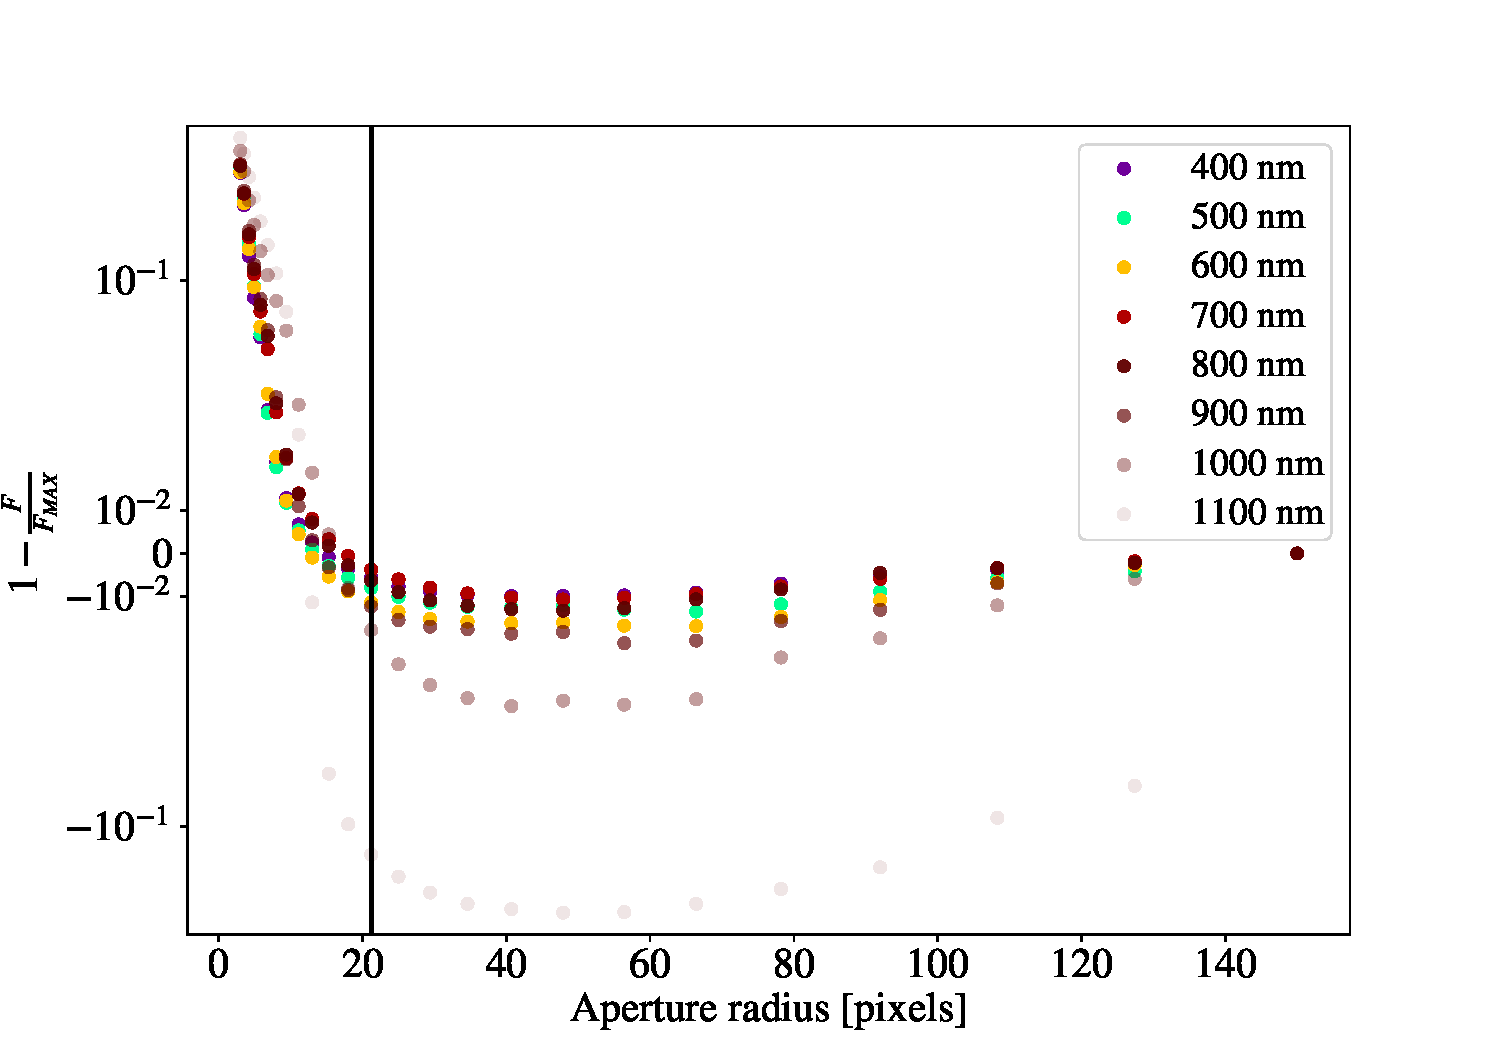
\includegraphics[width=\columnwidth]{fig/growth_curve_75um.pdf}
%    \caption{Growth curve obtained with the \spinhole pinhole. Le vertical axis is obtained by computing 1 minus the flux in ADU at the radius aperture in the horizontal axis $F$, normalized by the flux maximal at the maximal aperture $F_{MAX}$. Here the maximal aperture corresponds to a radius of 56.4 pixels. The scale is linear under 0.05, and logarithmic above.}
%    \label{fig:growth_75um}
%    %/stardice/analysis/cbp_paper/golden_sample_analysis/dr2/growth_curves.ipynb
%\end{figure}

\subsubsection{\bpinhole pinhole}

When using \bpinhole pinhole, the main spot take a significant area of the focal plane, meaning there is not enough background in the image to reconstruct it. We find the centroid of the spot of interest, and we measure the charges collected in the \SD camera by aperture photometry. We evaluate the optimal radius at 300 pixels for the \bpinhole pinhole in order to contain the main spot and the 1\up{st} order ghost (see growth curve figure \ref{fig:growth_5mm}). We estimate the background contribution by measuring the flux per pixel inside an annulus far from the main spot, between a internal radius of 420 pixels and an external radius of 470 pixels. This flux per pixel is multiplied by the surface of a disk of 300 pixels and subtracted to the flux of the main spot measured with aperture photometry. This quantity correspond to the charges $\Qccd$ collected in the \SD camera coming from the CBP with the \bpinhole pinhole.

%This time we use images without any light coming from the CBP to estimate the background. Between each image taken with light coming from the CBP, we took background images by turning off the laser. These background images were stationary with respect to time and wavelength, as it can be seen respectively in Figure~\ref{fig:stationarity_time} and \ref{fig:stationarity_wl}. We compute a master background by doing the mean from all of these background images. 
% We estimate the background by doing the aperture photometry at the same position and same radius of the master background, and then subtract it to the charge measured.
%The same method is applied for the \SI{2}{\milli\meter} pinhole, with an aperture of 150 pixels.

\begin{figure}[h]
    \centering
    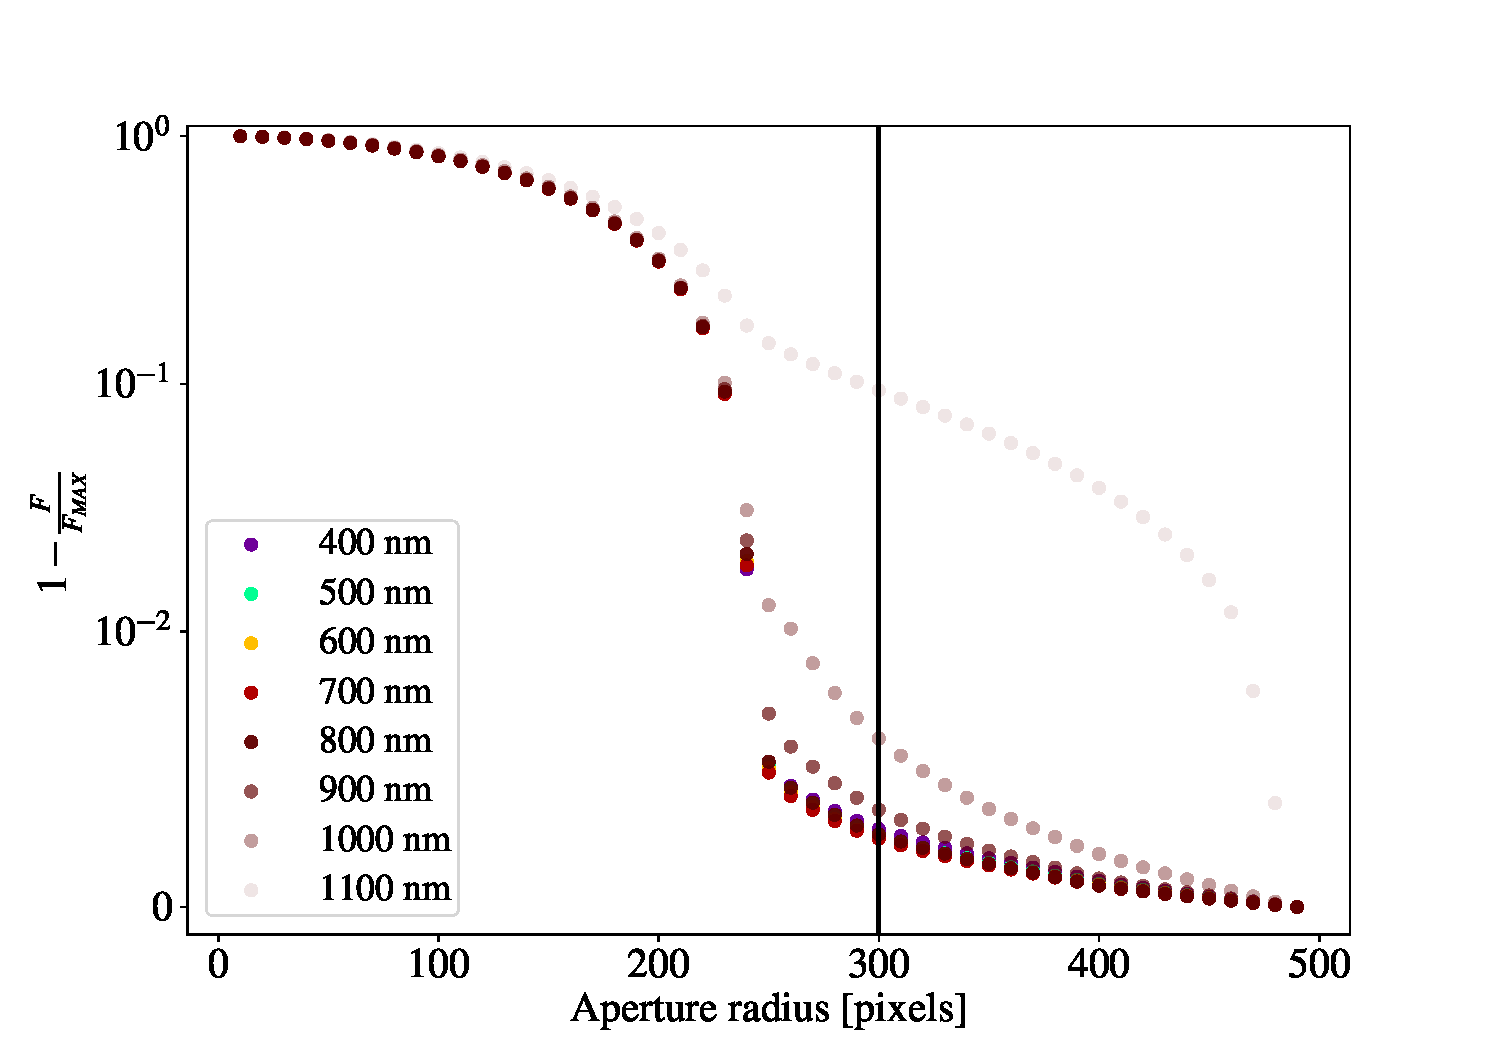
\includegraphics[width=\columnwidth]{fig/growth_curve_5mm.pdf}
    \caption{Growth curve obtained with the \spinhole pinhole. Le vertical axis is obtained by computing 1 minus the flux in ADU at the radius aperture in the horizontal axis $F$, normalized by the flux maximal at the maximal aperture $F_{MAX}$. Here the maximal aperture corresponds to a radius of 490 pixels. The scale is linear under 0.01, and logarithmic above.}
    \label{fig:growth_5mm}    
    %/stardice/analysis/cbp_paper/golden_sample_analysis/dr2/growth_curves.ipynb
\end{figure}

\begin{figure}[h]
    \centering
    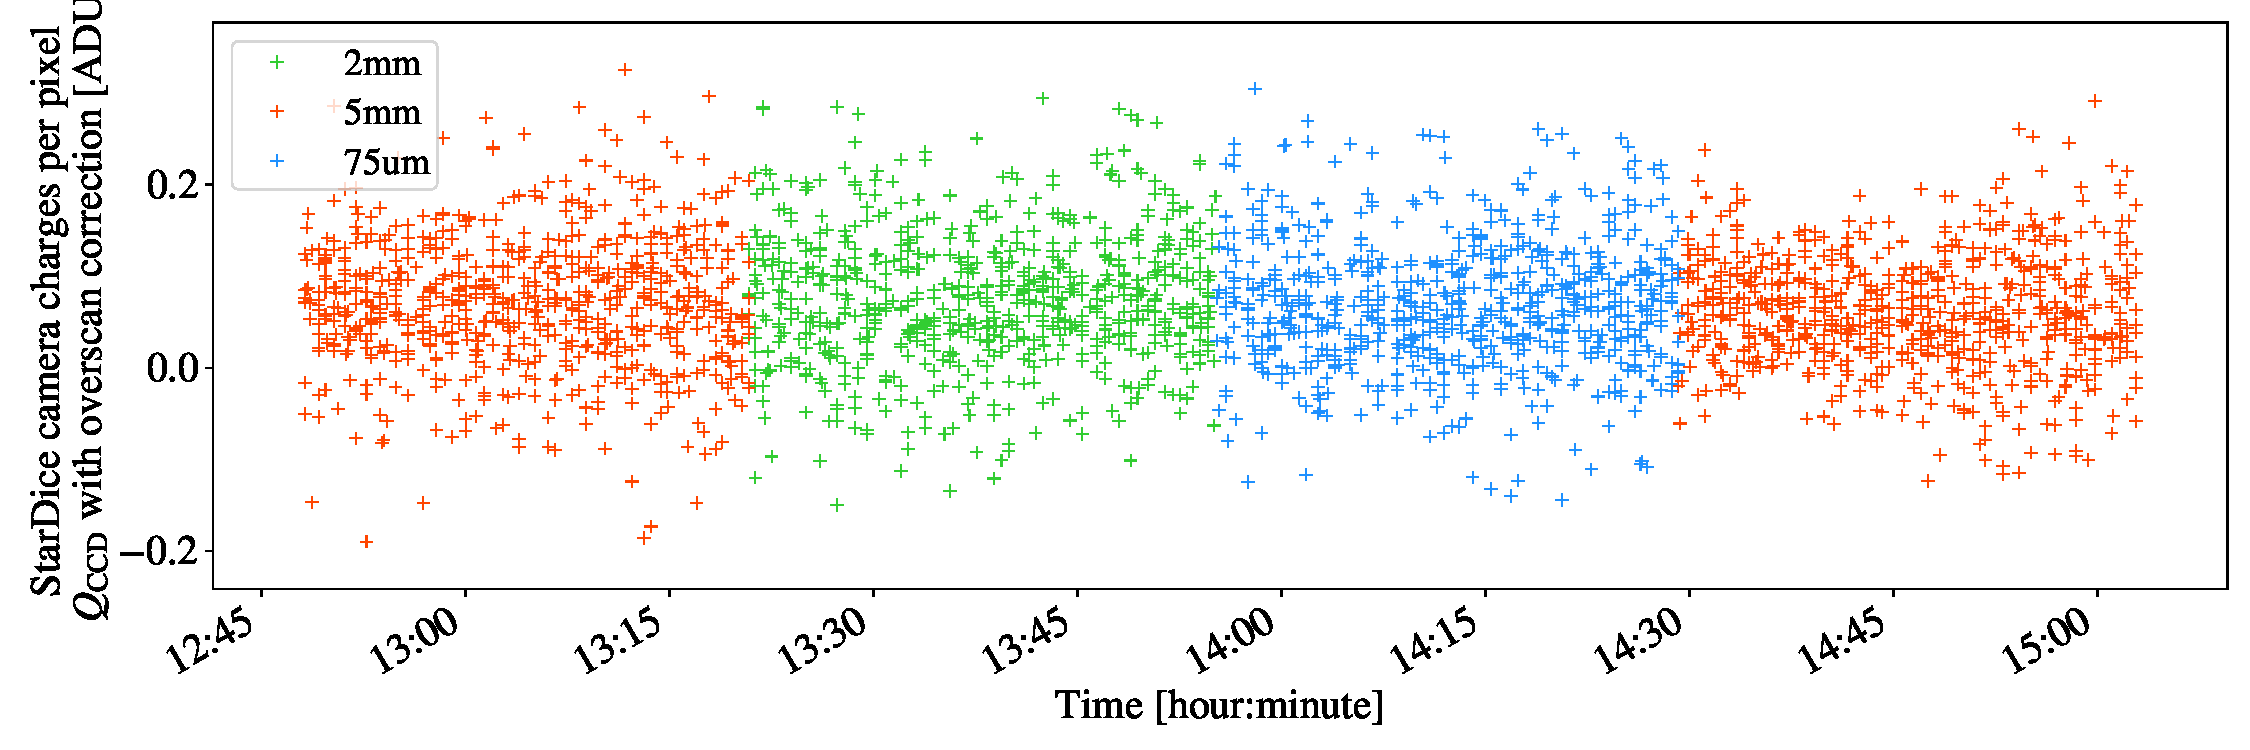
\includegraphics[width=\columnwidth]{fig/background_stationary_time.pdf}
    \caption{Charge per pixel for each background image in \SD with overscan correction with respect to the time.}
    \label{fig:stationarity_time}
    %/stardice/analysis/cbp_paper/golden_sample_analysis/dr2/background_and_centroid_stationarity.ipynb
\end{figure}
In Section~\ref{sec:strategy} we said that there is a need to change the pinhole in the CBP slides according to the measurement we want to do, as refered in Table~\ref{tab:schedule}. We need to ensure that we understand how the CBP response has changed when we switched the pinhole. 
\begin{figure}[h]
    \centering
    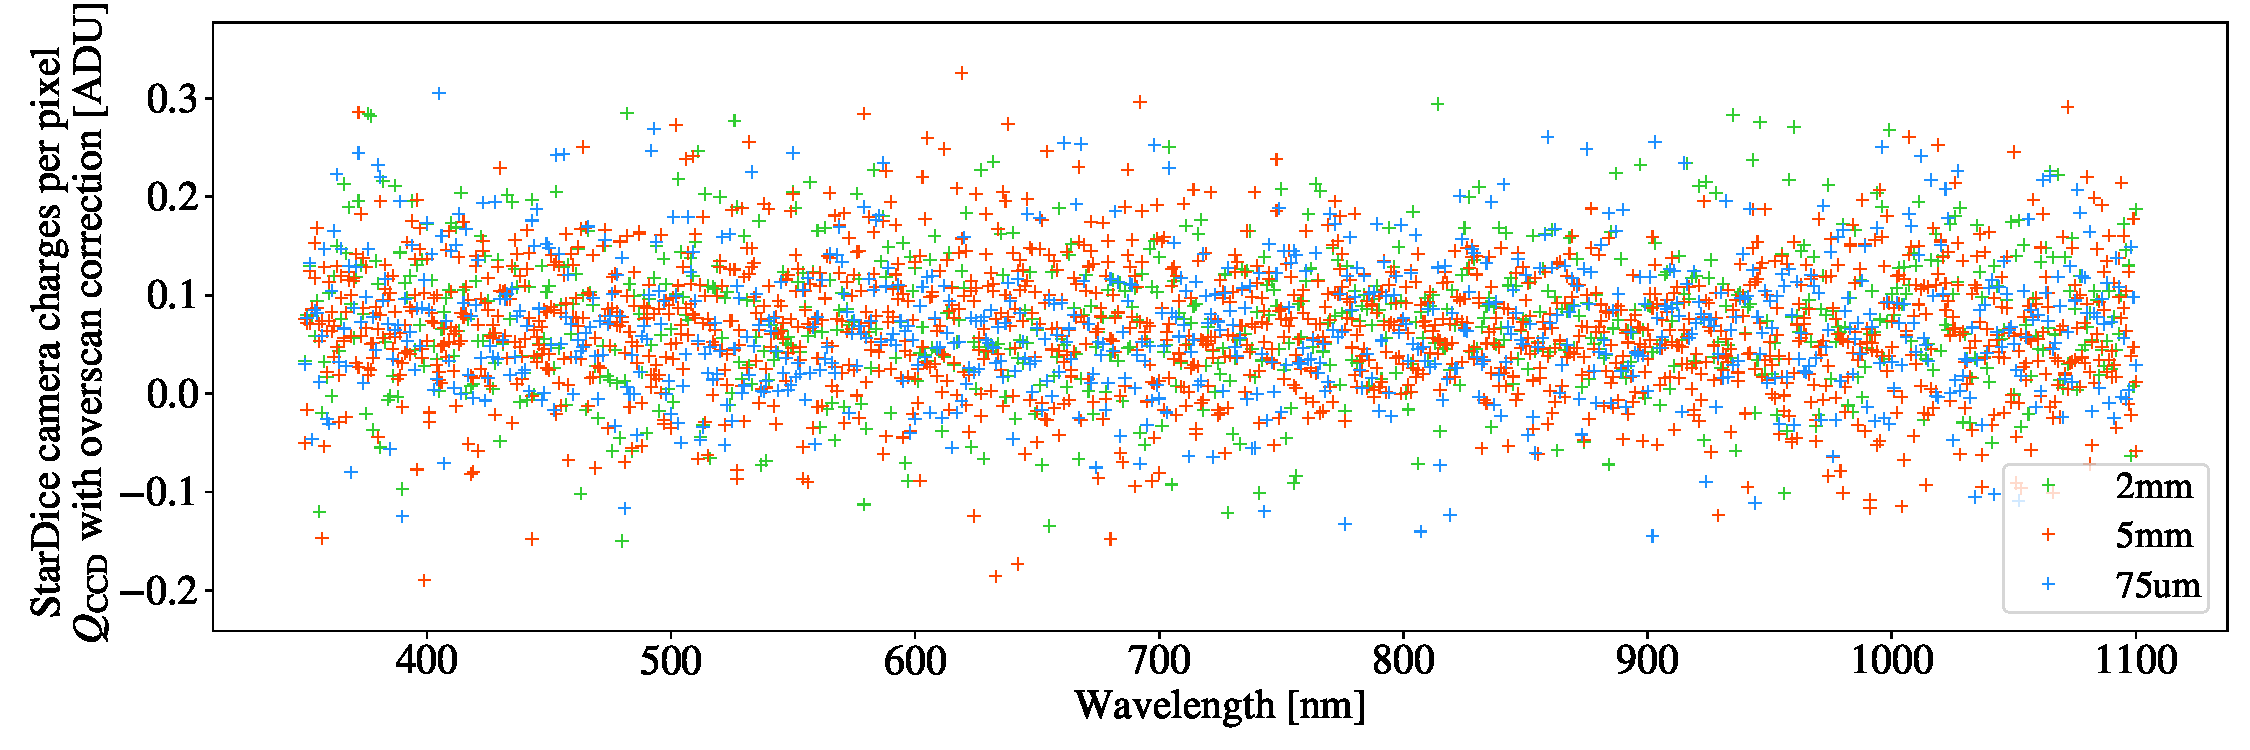
\includegraphics[width=\columnwidth]{fig/background_stationary_wavelength.pdf}
    \caption{Charge per pixel for each background image in \SD with overscan correction with respect to the wavelength.}
    \label{fig:stationarity_wl}
\end{figure}


\subsection{Correction of the ghost contamination}

In Section~\ref{sec:strategy} we discussed the need to intercalibrate the CBP response for both pinhole sizes. To this purpose, we took measurements with the \SD telescope with both \bpinhole pinhole and \spinhole pinhole, and evaluate the systematic related to this change of pinhole diameter. One major difference between the \spinhole pinhole and the \bpinhole pinhole is how the ghost and the main spot superimpose on the focal plane. We show in Figure~\ref{fig:schema_ghost} the optical path that produces the 1\up{st} order ghost on the focal plane. In Figure~\ref{fig:ghost_contrast}, we can see an image of the 1\up{st} order ghost next to the main spot obtained with the \spinhole pinhole. The distance between the centroïd of the main spot and the centroïd of the 1\up{st} order ghost is between 30 to 70 pixels depending on the radial position on the mirror. In the mean time, the \bpinhole pinhole photometry is made with an aperture of 300 pixels, containing the 1\up{st} order ghost and the main spot. We need to know the fraction of the flux that corresponds to the 1\up{st} order ghost.


\begin{figure}[h]
    \centering
    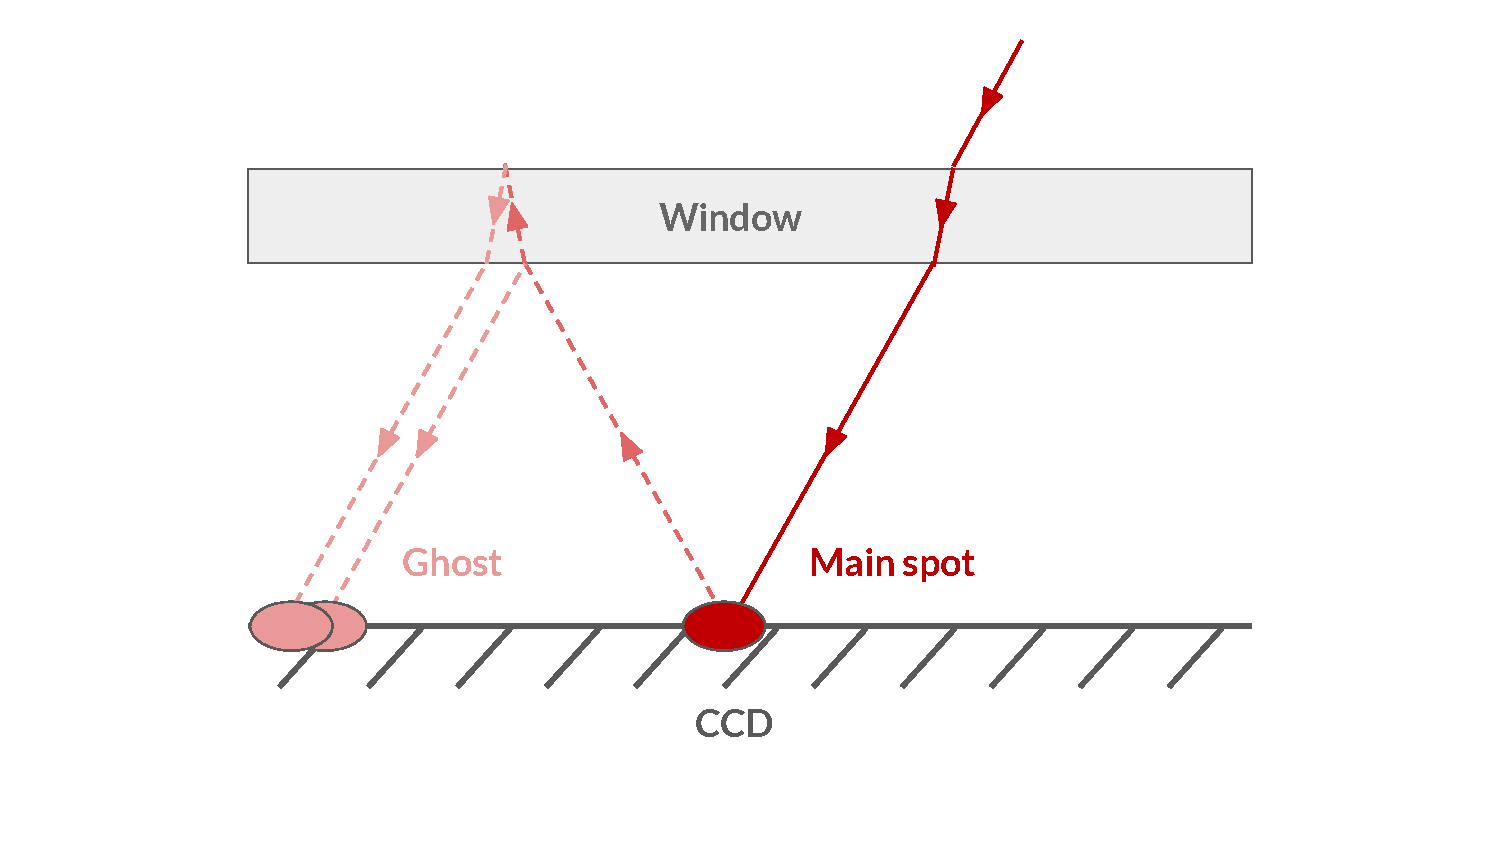
\includegraphics[width=\columnwidth]{fig/schema_ghost.pdf}
    \caption{Schematic of the origin of the 1\up{st} order ghost. A fraction of the incident light reflects on the surface of the CCD, and then reflects again on one of the two faces of the window, and are then absorbed by the CCD. This creates a defocused and less intense image at an other position in the focal plane. Everytime light is absorbed by the CCD, a fraction is reflected and generate a new ghost farther.}
    \label{fig:schema_ghost}
    %~/stardice/analysis/cbp_paper/golden_sample_analysis/dr2/ghost_photometry_general.ipynb
\end{figure}


\begin{figure}[h]
    \centering
    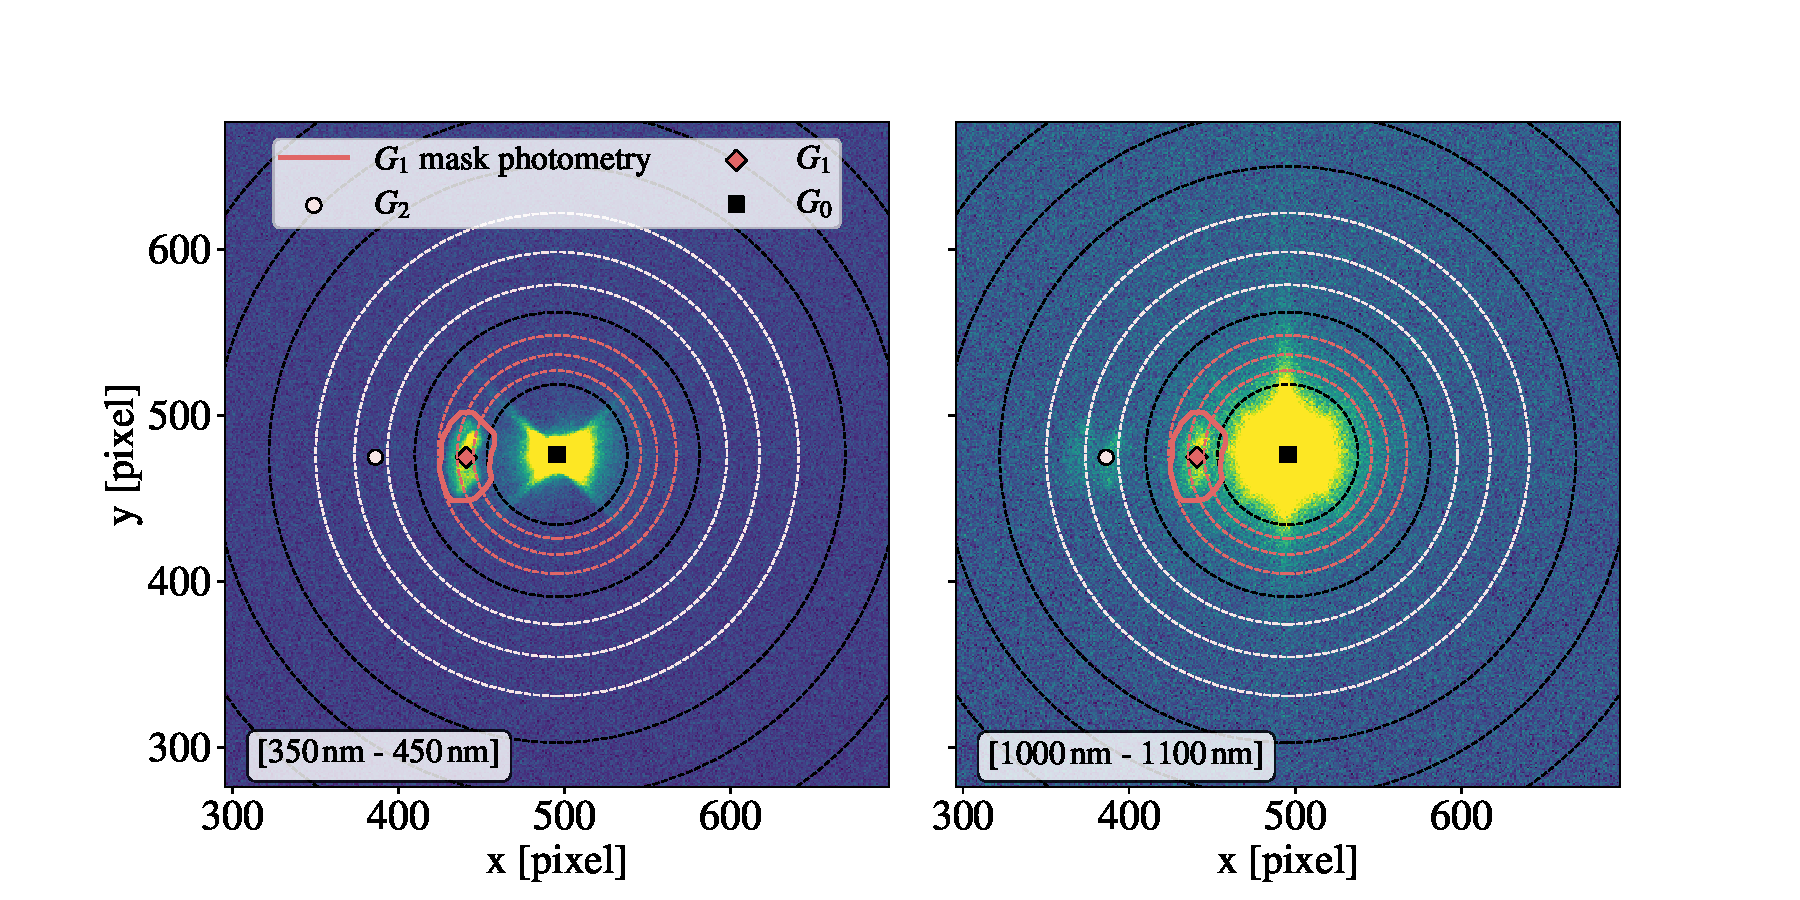
\includegraphics[width=\columnwidth]{fig/ghost_contrast.pdf}
    \caption{Image of the main spot in the center and the first order ghost at its left. The level max of the color bar is set low intentionally to make the ghost visible. The distance between the first order ghost and the main spot is between 30 and 70 pixels depending on the radial position of the point of impact on the \SD primary mirror.}
    \label{fig:ghost_contrast}
    %~/stardice/analysis/cbp_paper/golden_sample_analysis/dr2/ghost_photometry_general.ipynb
\end{figure}


\subsubsection{First order ghost photometry}

We want to quantify the contribution of the ghost relatively to the main spot for the \bpinhole pinhole. Let be $G_0(\lambda)$ the quantity of light collected in the main spot, and $G_\mathrm{n}(\lambda)$ the quantity of light collected in the ghost of order $n$. We define $\Kghost(\lambda)$ the ratio of the 1\up{st} order ghost $G_1(\lambda)$ over the main spot $G_0(\lambda)$:

\begin{equation}
    \Kghost = \frac{G_1(\lambda)}{G_0(\lambda)}
    \label{eq:ratio_ghost}
\end{equation}

We make the hypothesis that the ratio $\Kghost(\lambda)$ is the same for both pinholes. We measure $G_1(\lambda)$ with the \spinhole pinhole where it is well separated from $G_0(\lambda)$. We build a mask with the expected ghost shape and we fit its best position on the image. $G_1(\lambda)$ is the sum of the ADUs contained in this mask, after background subtraction. To estimate the background at this position, we assume that the main spot has a spatial vertical symmetry. We place a symmetric mask at the vertical symmetric position and measure the ADUs contained inside, which correspond to background only. This background is subtracted to the photometry of the 1\up{st} order ghost to obtain $G_1(\lambda)$. On the other hand, $G_0(\lambda)$ is measured with the aperture photometry described in \ref{sec:photometry}. The results obtained for $\Kghost(\lambda)$ for 5 different measurements are shown in Figure~\ref{fig:ghost_ratio}.


 \begin{figure}[h]
     \centering
     \resizebox{\hsize}{!}{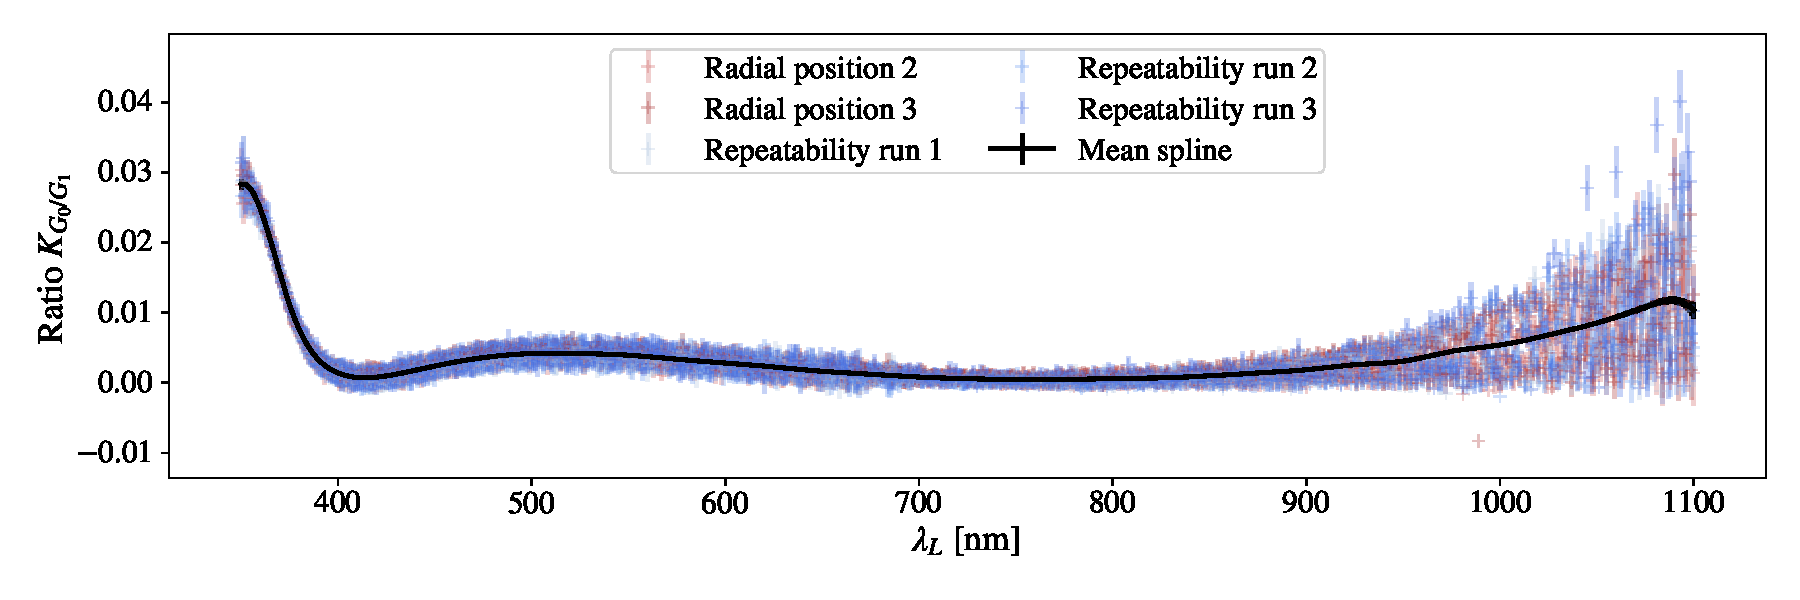
\includegraphics{fig/ghost_ratio.pdf}}
     \caption{Ratio $\Kghost$ (which correspond to the order 1 ghost $G_{1}(\lambda)$ over the main spot $G_0(\lambda)$) with respect to $\lambda_L$. The mean spline goes through five datasets, three at the same position on the mirror, two other at a different radial position on the mirror. All responses are at the same position on the focal plane.}
     \label{fig:ghost_ratio}
    %~/stardice/analysis/cbp_paper/golden_sample_analysis/dr2/ghost_photometry_general.ipynb
 \end{figure}
 
 \subsubsection{Contribution of the n\up{th} order ghosts}

Now that we did the photometry for the first order ghost, we want to estimate the contribution of higher orders. Since the intensity of these ghosts is very weak and hard to analyse, we simulate their contribution from the $1^{\mathrm{st}}$ order ghost analysis. Let be $\Rwindow$ the reflection coefficient at the interface air-window, and $\Rccd$ the reflection coefficient at the interface air-CCD. We know the transmission of the window $T_\mathrm{window}(\lambda)$ from manufacturer datasheets, so we can infer $\Rwindow$:
 
\begin{equation}
    \Rwindow = 1 - T_\mathrm{window}(\lambda).
    \label{eq:rwindow}
\end{equation}
 
\noindent We define $F$ the flux collected by the camera, $G_0(\lambda)$ the quantity of light collected in the main spot, and $G_\mathrm{n}(\lambda)$ the quantity of light collected in the ghost of order $n$. $G_0(\lambda)$ and $G_\mathrm{n}(\lambda)$ are a function of F: 

\begin{equation}
     G_0(\lambda) = (1-\Rwindow)^{2} \times (1-\Rccd) \times F, 
     \label{eq:g0}
\end{equation}

\begin{equation}
\begin{aligned}
    G_\mathrm{n}(\lambda) & = G_{0}(\lambda) \times [\Rccd \Rwindow + \Rccd(1-\Rwindow)\Rwindow]^{n} \\
    & = G_{0}(\lambda) \times [2 \Rccd \Rwindow - \Rccd \Rwindow^{2}] ^{n}. \\
     \label{eq:gn}
\end{aligned}
\end{equation}

\noindent The sum of all the ghosts $G_{\mathrm{n>0}}(\lambda)$ is defined as
\footnote{If |q| < 1, the serie $\left( \sum_{n=0}^{m} q^n \right)_{\mathrm{m \in \mathbb{N}}}$ strictly converge and \\ $\sum_{n=0}^{\infty} q^n \equiv \lim\limits_{m \rightarrow \infty} \sum_{n=0}^{m} q^n = \frac{1}{1-q}$}:

 \begin{equation}
 \begin{aligned}
     G_{n>0}(\lambda) & = \sum_{n=0}^{\mathrm{n} \rightarrow \infty} G_\mathrm{n}(\lambda) - G_0(\lambda) \\
     & = G_0(\lambda) \times \sum_{n=0}^{n \rightarrow \infty} \left( [2 \Rccd \Rwindow - \Rccd \Rwindow^{2}] ^{n} - G_0(\lambda) \right)\\
     & = G_0(\lambda) \times\left( \frac{1}{1- [2 \Rccd \Rwindow - \Rccd \Rwindow^{2}]} - 1\right),
     \label{eq:sum_ghost}
 \end{aligned}
 \end{equation}
 
\noindent and the sum of the ghost of order higher than 1 is defined as:

 \begin{equation}
     G_{n>1}(\lambda) = G_{n>0}(\lambda) - G_1(\lambda).
     \label{eq:sum_ghost_sup_1}
 \end{equation}

\noindent As we measure the photometry of the 1\up{st} order ghost $G_1(\lambda)$, we want to verify that the ghosts of higher orders $G_{\mathrm{n}>1}(\lambda)$ are negligible. Using the Equations~\ref{eq:ratio_ghost}, \ref{eq:g0} and \ref{eq:gn}, we can compute $\Rccd$:

\begin{equation}
    \Rccd = \frac{\Kghost}{\Rwindow (2 - \Rwindow)}.
    \label{eq:rccd}
\end{equation}

We measured $G_1(\lambda)$ with photometry, and estimate $G_{\mathrm{n}>1}$ with the equations above. We show the ratio $K_{G_{\mathrm{n}>1}/G_0}$ in Figure~\ref{fig:ratio_ginf_g0}, and we see that $K_{G_{\mathrm{n}>1}/G_0}$ is always below the per mil level. Since $G_{\mathrm{n}>1}$ contribute for less than a per mil of $G_0(\lambda)$, we decide to neglect it.

\begin{figure}[h]
    \centering
    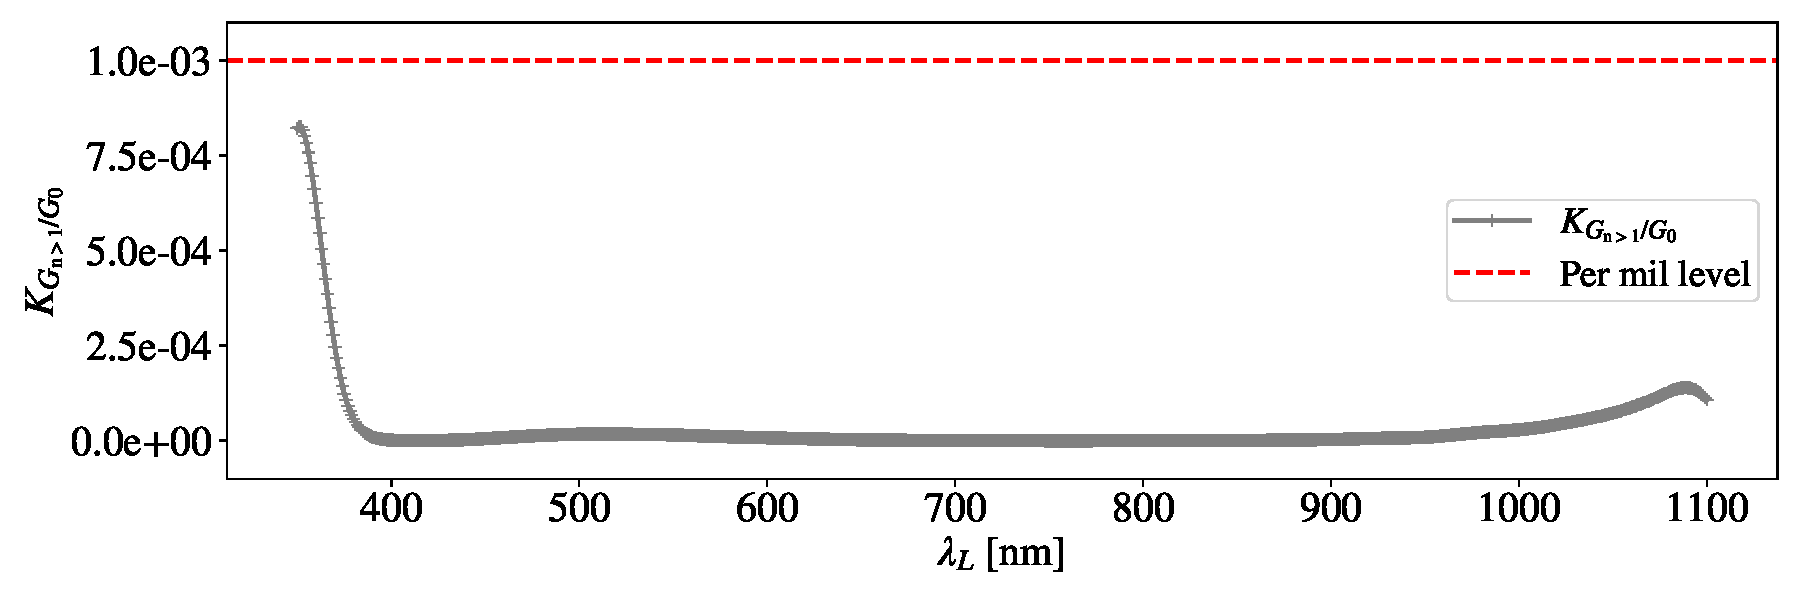
\includegraphics[width=\columnwidth]{fig/ratio_g1_ginf.pdf}
    \caption{Ratio $K_{G_{\mathrm{n}>1}/G_0}(\lambda)$ (which correspond to the sum of the ghosts at order higher than 1 $G_{\mathrm{n}>1}(\lambda)$ over $G_0(\lambda)$) with respect to $\lambda_L$.}
    \label{fig:ratio_ginf_g0}
    %~/stardice/analysis/cbp_paper/golden_sample_analysis/dr2/ghost_convergence.ipynb   
\end{figure}

\subsubsection{Ghost contribution for \bpinhole pinhole}

The total charges $\Qccd{}_{, \, \SI{5}{\milli\meter}}(\lambda)$ measured by doing the aperture photometry at 300 pixels for the \bpinhole pinhole is the sum of the charges $Q_0(\lambda)$ in the main spot $G_0(\lambda)$ and the charges $\Qghost(\lambda)$ in the 1\up{st} order ghost $G_1(\lambda)$. With $\Eccd$ the quantum efficiency of the StarDICE CCD camera, we define these quantites as:

\begin{equation}
    \Qghost(\lambda) = G_1(\lambda) \times \Eccd, 
    \label{eq:qghost}
\end{equation}

\begin{equation}
    Q_0(\lambda) = G_0(\lambda) \times \Eccd.
    \label{eq:qmain}
\end{equation}

\noindent Then $Q_0(\lambda)$ can be measured as follow:

\begin{equation}
\begin{aligned}
    Q_0(\lambda) & = \Qccd{}_{, \, \SI{5}{\milli\meter}}(\lambda) - \Qghost(\lambda) \\
    & = \frac{\Qccd{}_{, \, \SI{5}{\milli\meter}}(\lambda)}{1 + \Kghost(\lambda)}.
    \label{eq:qccd_5mm}
\end{aligned}
\end{equation}

\noindent Now that we have a good estimation of the flux for the 

\noindent Once we have corrected the \bpinhole pinhole from the ghost contribution, we can compute the ratio between the \SD responses defined as $\Kpinholes(\lambda)$ in Equation~\ref{eq:ratio_pinholes}. Thanks to this equation, we can infer $\Rcbp^{\spinhole}(\lambda)$ from the measurement of $\Rcbp^{\bpinhole}(\lambda)$.

\begin{equation}
    \Kpinholes(\lambda) = \frac{\Rcbp^{\bpinhole}(\lambda)}{\Rcbp^{\spinhole}(\lambda)}
    \label{eq:ratio_pinholes}
\end{equation}

We show these ratios before and after the ghost correction in the upper Figure~\ref{fig:ratio_pinholes}. We expect the ratio to be linear since it should be the ratio of two surfaces, so we draw a linear spline through the data. In the ultraviolet below \SI{400}{\nm} where the window is highly reflective, we see that the ghost correction has flattened the ratios. Above \SI{900}{\nm} we can see a significative difference between the ratio and the linear spline. This phenomenon is not quite understood and is discussed in section \ref{sec:discussion}, but we precise that the linear fit is made only for the wavelengths below \SI{900}{\nano\meter}. 

\begin{figure}[h]
    \centering
    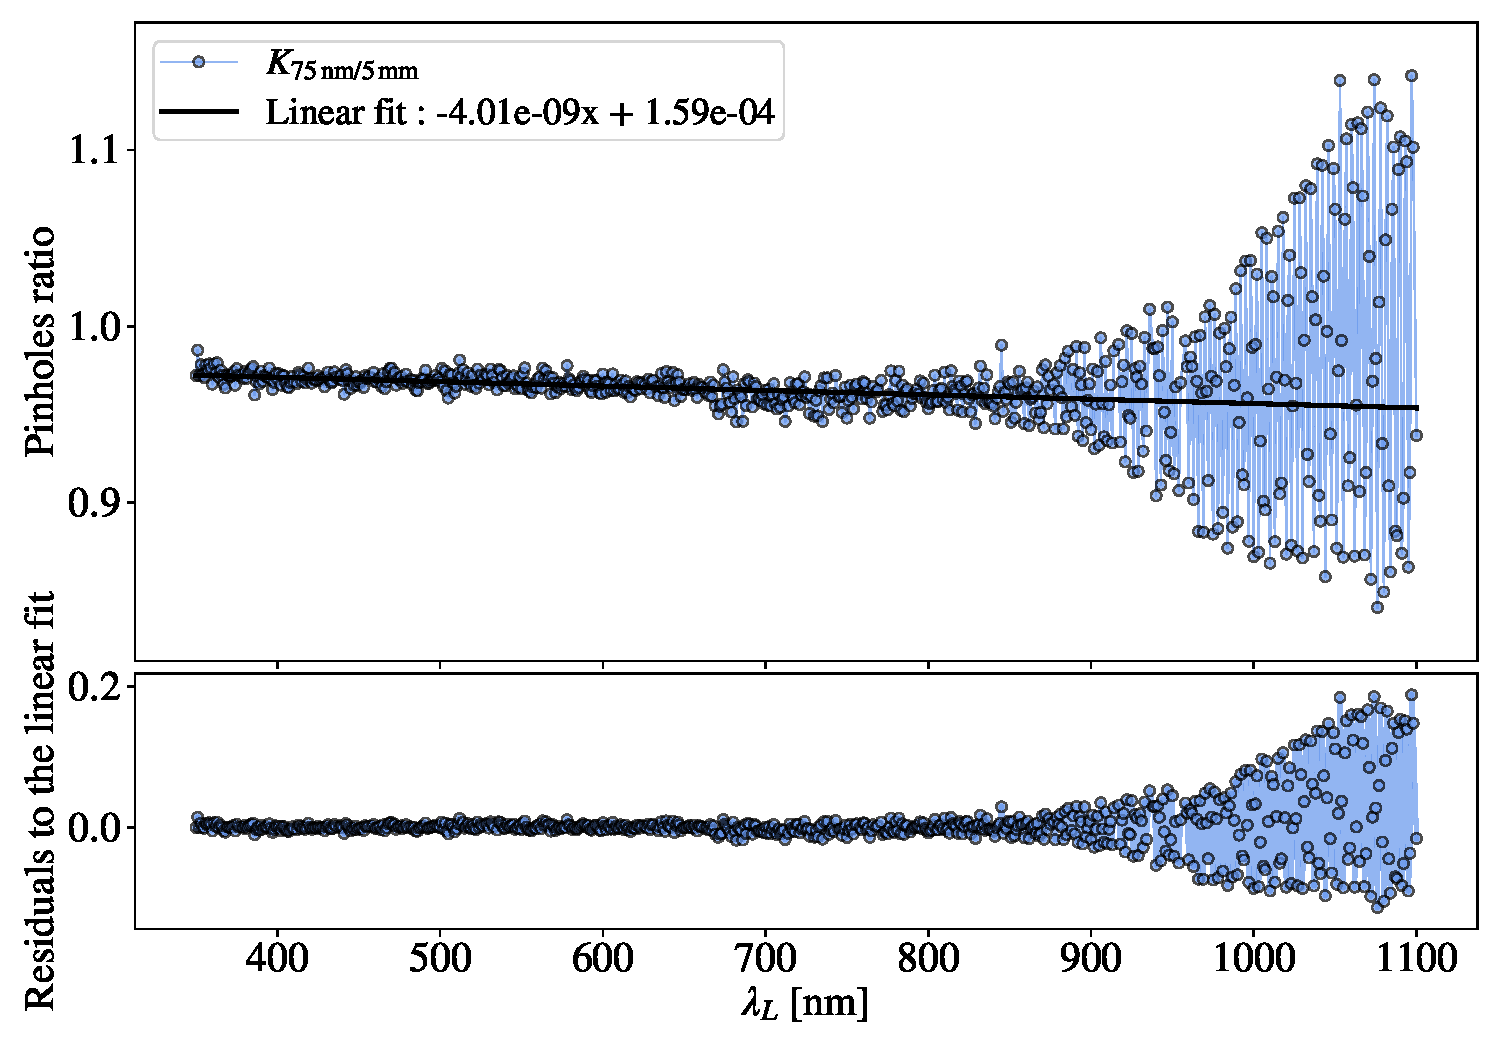
\includegraphics[width=\columnwidth]{fig/ratio_pinholes.pdf}
    \caption{Ratio $\Kpinholes(\lambda)$ with respect to wavelength, before and after ghost correction. We compute a linear spline that best fit the data between \SI{400}{\nm} and \SI{900}{\nm}.}
    \label{fig:ratio_pinholes}
    %~/stardice/analysis/cbp_paper/golden_sample_analysis/dr2/ratio_pinholes.ipynb
\end{figure}

\subsubsection{Summary}

The summary of the error budget on the \SD telescope response id detailed in Figure~\ref{fig:sd_budget}


\begin{figure}
    \centering
    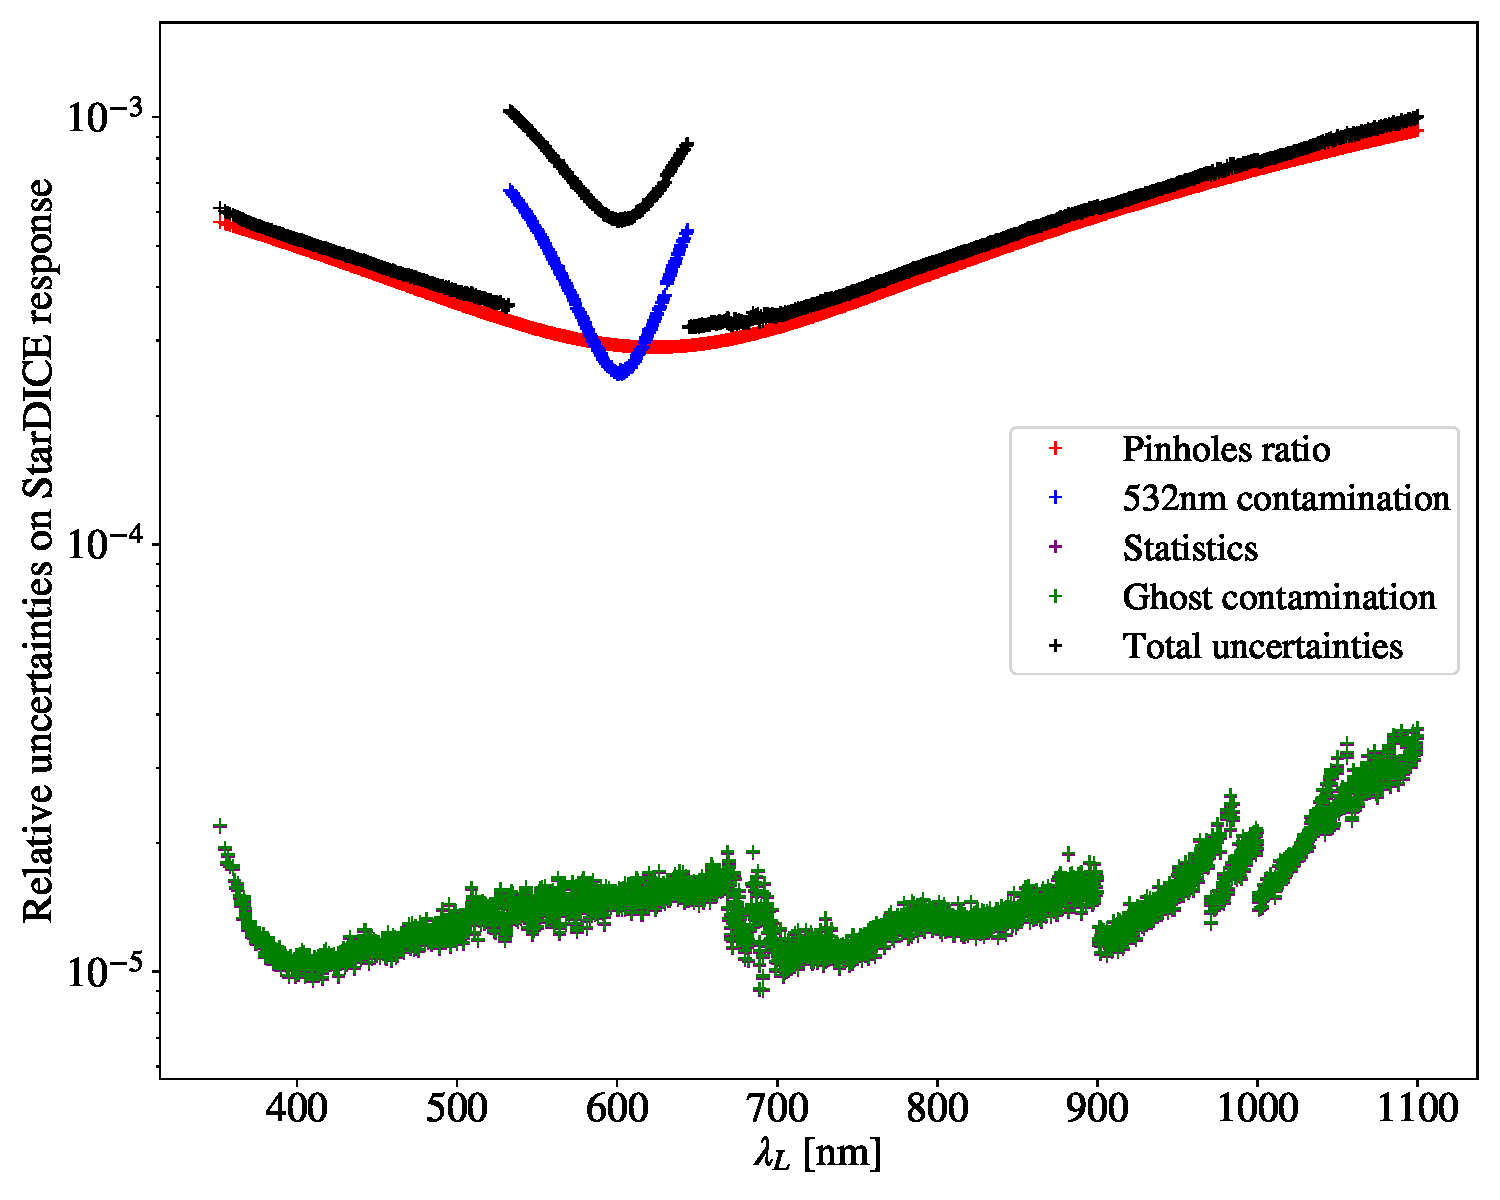
\includegraphics[width=\columnwidth]{fig/sd_uncertainties_budget.pdf}
    \caption{Total error budget for \SD response.}
    \label{fig:sd_budget}
\end{figure}


\subsection{Correction of the light contamination}\label{sec:sd_contaminations}

When extracting the charges from the \SD camera, we have to remove light contaminations described in Sections~\ref{sec:532_cont} and~\ref{sec:fluorescence}. As the photodiode and the solar cell, the total charge measured in the \SD camera $\Qccdmes$ is the sum of the charges from the main laser line $\Qccdcal$ and the charges from the \SI{532}{\nm} contamination $\Qccd^{532}$, the $\lambda_{\rm comp}$ contamination $\Qccd^{\lambda_{\rm comp}}$, and the integrating sphere fluorescence $\Qccd^{\mathrm{fluo}}$, as follows:
\begin{equation}
    \Qccdmes = \Qccdcal + \Qccd^{532} + \Qccd^{\lambda_{\rm comp}} + \Qccd^{\mathrm{fluo}}
    \label{eq:qccd_mes}
\end{equation}

As we defined the final calibrated amount of charges detected in the solar cell $\Qsolarcal$, we do the same with the \SD CCD. The light detected by the \SD CCD has gone through the CBP optics and the \SD telescope. These instruments have respectively optical responses defined as $\Rcbp(\lambda)$ and $\Rtel(\lambda)$. We can define $R(\lambda)$ the total response of the CBP and the \SD telescope optics:
\begin{equation}
    R(\lambda) = \Rtel(\lambda) \times \Rcbp(\lambda).
    \label{eq:rtot}
\end{equation}
Then, the contamination contribution in \SD camera from every source is evaluated multiplying photodiode charge contamination by $R(\lambda)$.
The impact of these subtractions is illutrated in Figure~\ref{fig:g_filter_532} focusing on the \SD g filter, the most affected filter by integrating sphere fluorescence and \SI{532}{\nano\meter} line.

\begin{figure}[h]
    \centering
    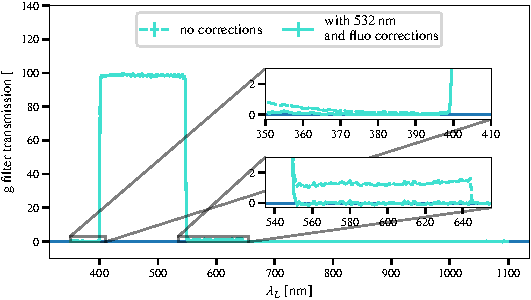
\includegraphics[width=\columnwidth]{fig/g_filter_532.pdf}
    \caption{StarDice g filter transmission as a function of the set laser wavelength $\lambda_L$, with and without the \SI{532}{\nm} correction. For clarity, we added a zoom on the out-of-band transmission where $\SI{532}{\nm}$ line is transmitted while higher wavelengths are shot by the laser.}
    \label{fig:g_filter_532}
    %cbp_paper_plots.ipynb
\end{figure}

\subsection{\SD response scan}

\subsubsection{\SD optics, filters and grating responses}

In this section we present the results of our different measurements. The following measurements are all taken at the same position on the mirror and the focal plane. The Figure~\ref{fig:stardice_5mm_response} show the \SD response obtained with the \bpinhole pinhole, and no filter. The Figure~\ref{fig:stardice_75um_response} show the \SD response obtained with the \spinhole pinhole, with all filters. In this figure we have a wavelength resolution sufficient enough to see the filter edges. The Figure~\ref{fig:stardice_grating_response} show the \SD response obtained with the \spinhole pinhole, with the grating set in front of the camera. The grating being blazed so that the 1\up{st} order of diffraction is the brightest, so we will mainly focus on this order of diffraction. We see a cut of the 2\up{nd} and 3\up{rd} order that correspond to the wavelength at which the signal is outside the CCD sensor.

\begin{figure}[h]
    \centering
    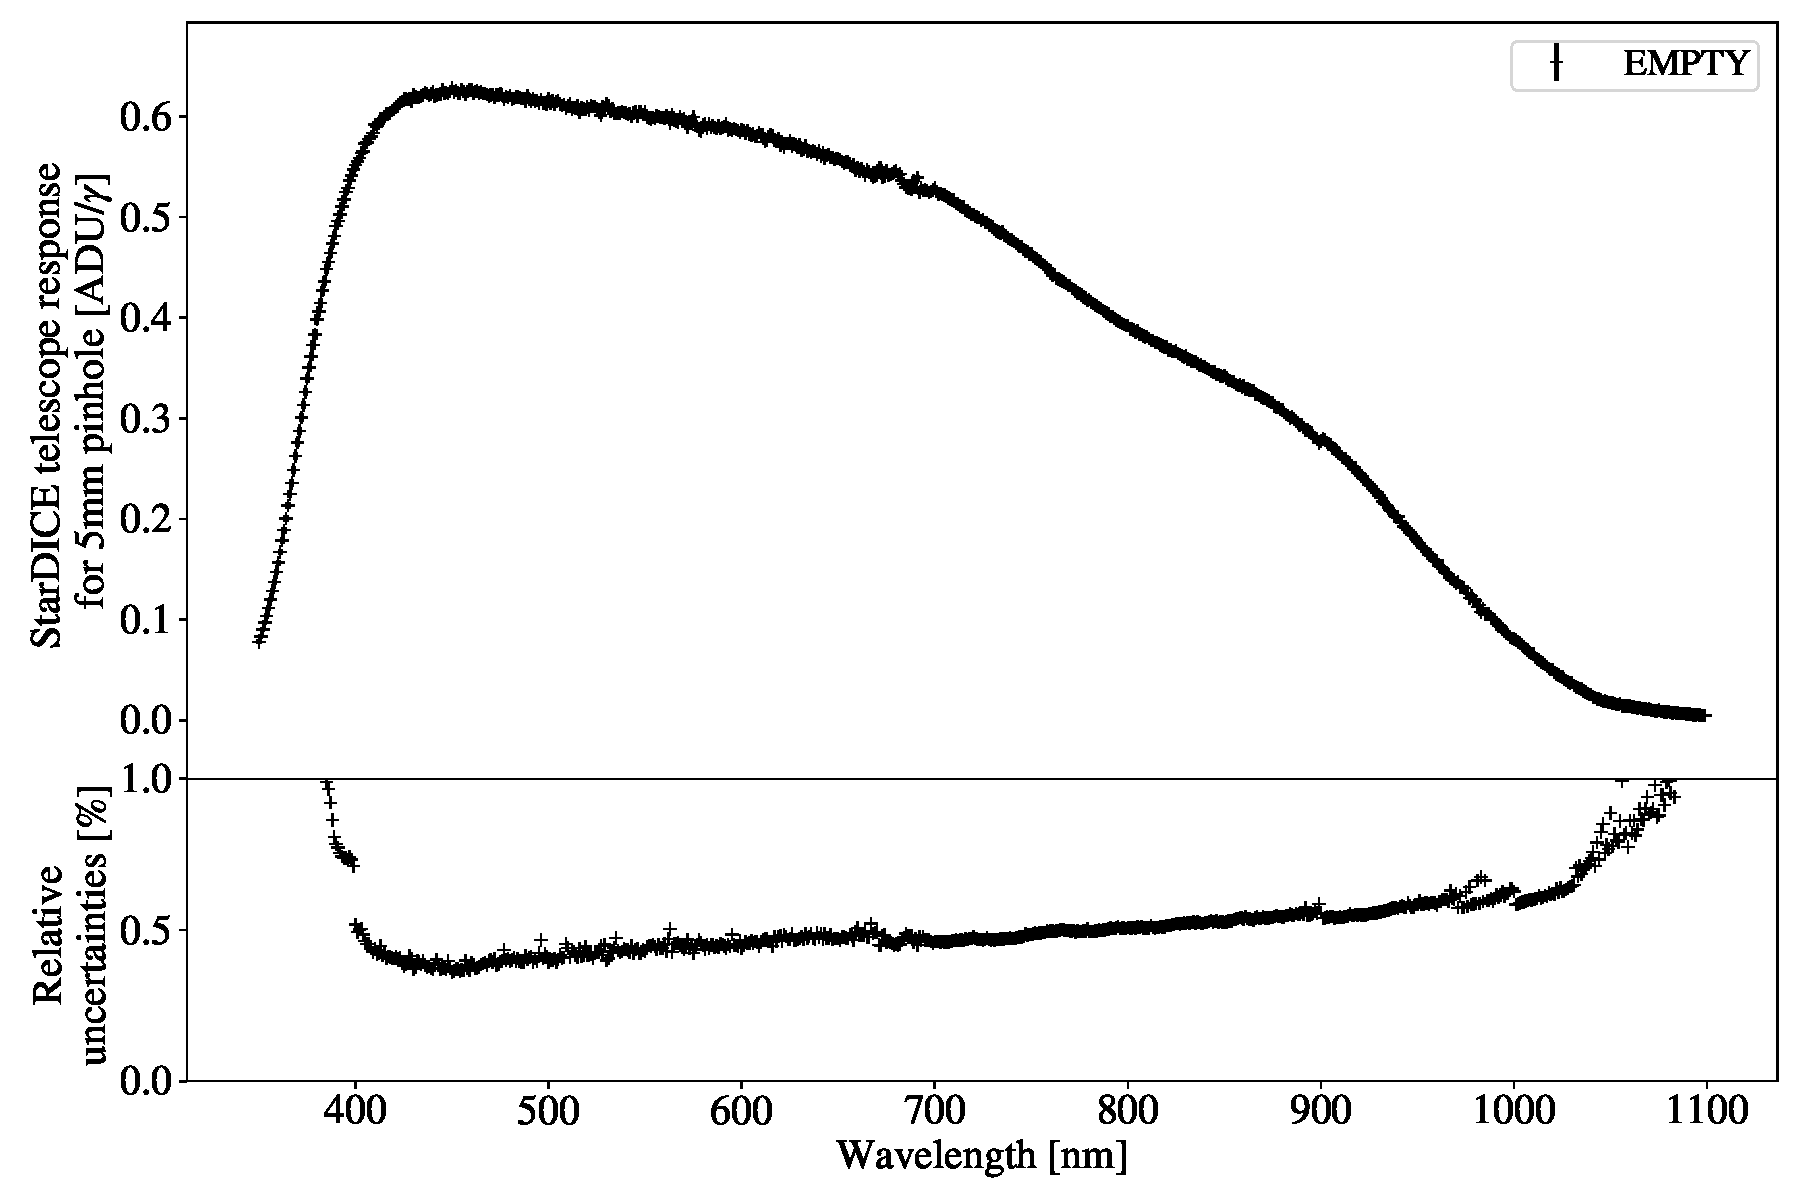
\includegraphics[width=\columnwidth]{fig/stardice_5mm_response.pdf}
    \caption{Up : \SD response with no filter and \bpinhole pinhole with respect to wavelength in nanometer. Bottom : Uncertainties over the \SD response measurement with respect to wavelength in nanometer.}
    \label{fig:stardice_5mm_response}
    %~/stardice/analysis/cbp_paper/golden_sample_analysis/dr2/response_plots.ipynb
\end{figure}

\begin{figure}[h]
    \centering
    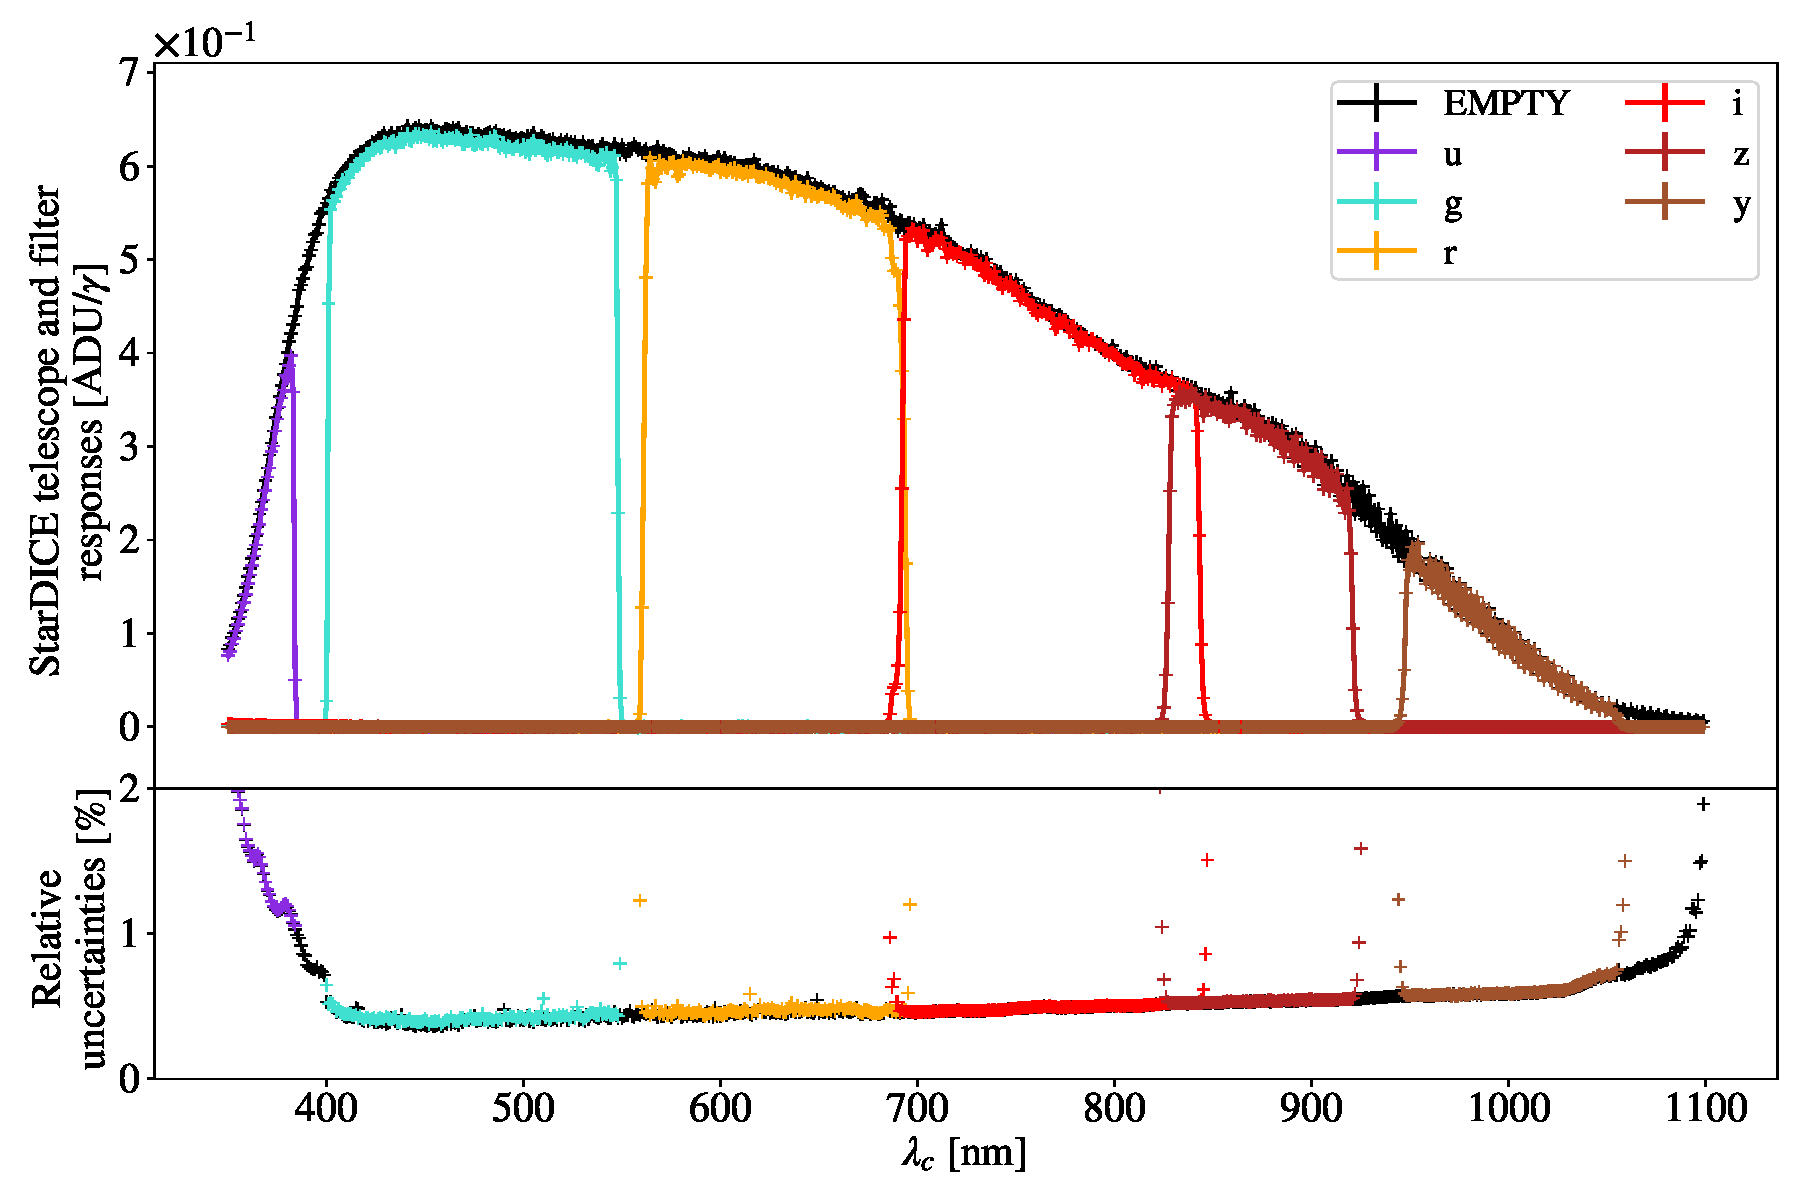
\includegraphics[width=\columnwidth]{fig/stardice_75um_response.pdf}
    \caption{Up : \SD response with at all filters and \spinhole pinhole with respect to wavelength in nanometer. Bottom : Uncertainties over the \SD response measurement with respect to wavelength in nanometer.}
    \label{fig:stardice_75um_response}
    %~/stardice/analysis/cbp_paper/golden_sample_analysis/dr2/response_plots.ipynb
\end{figure}

\begin{figure}[h]
    \centering
    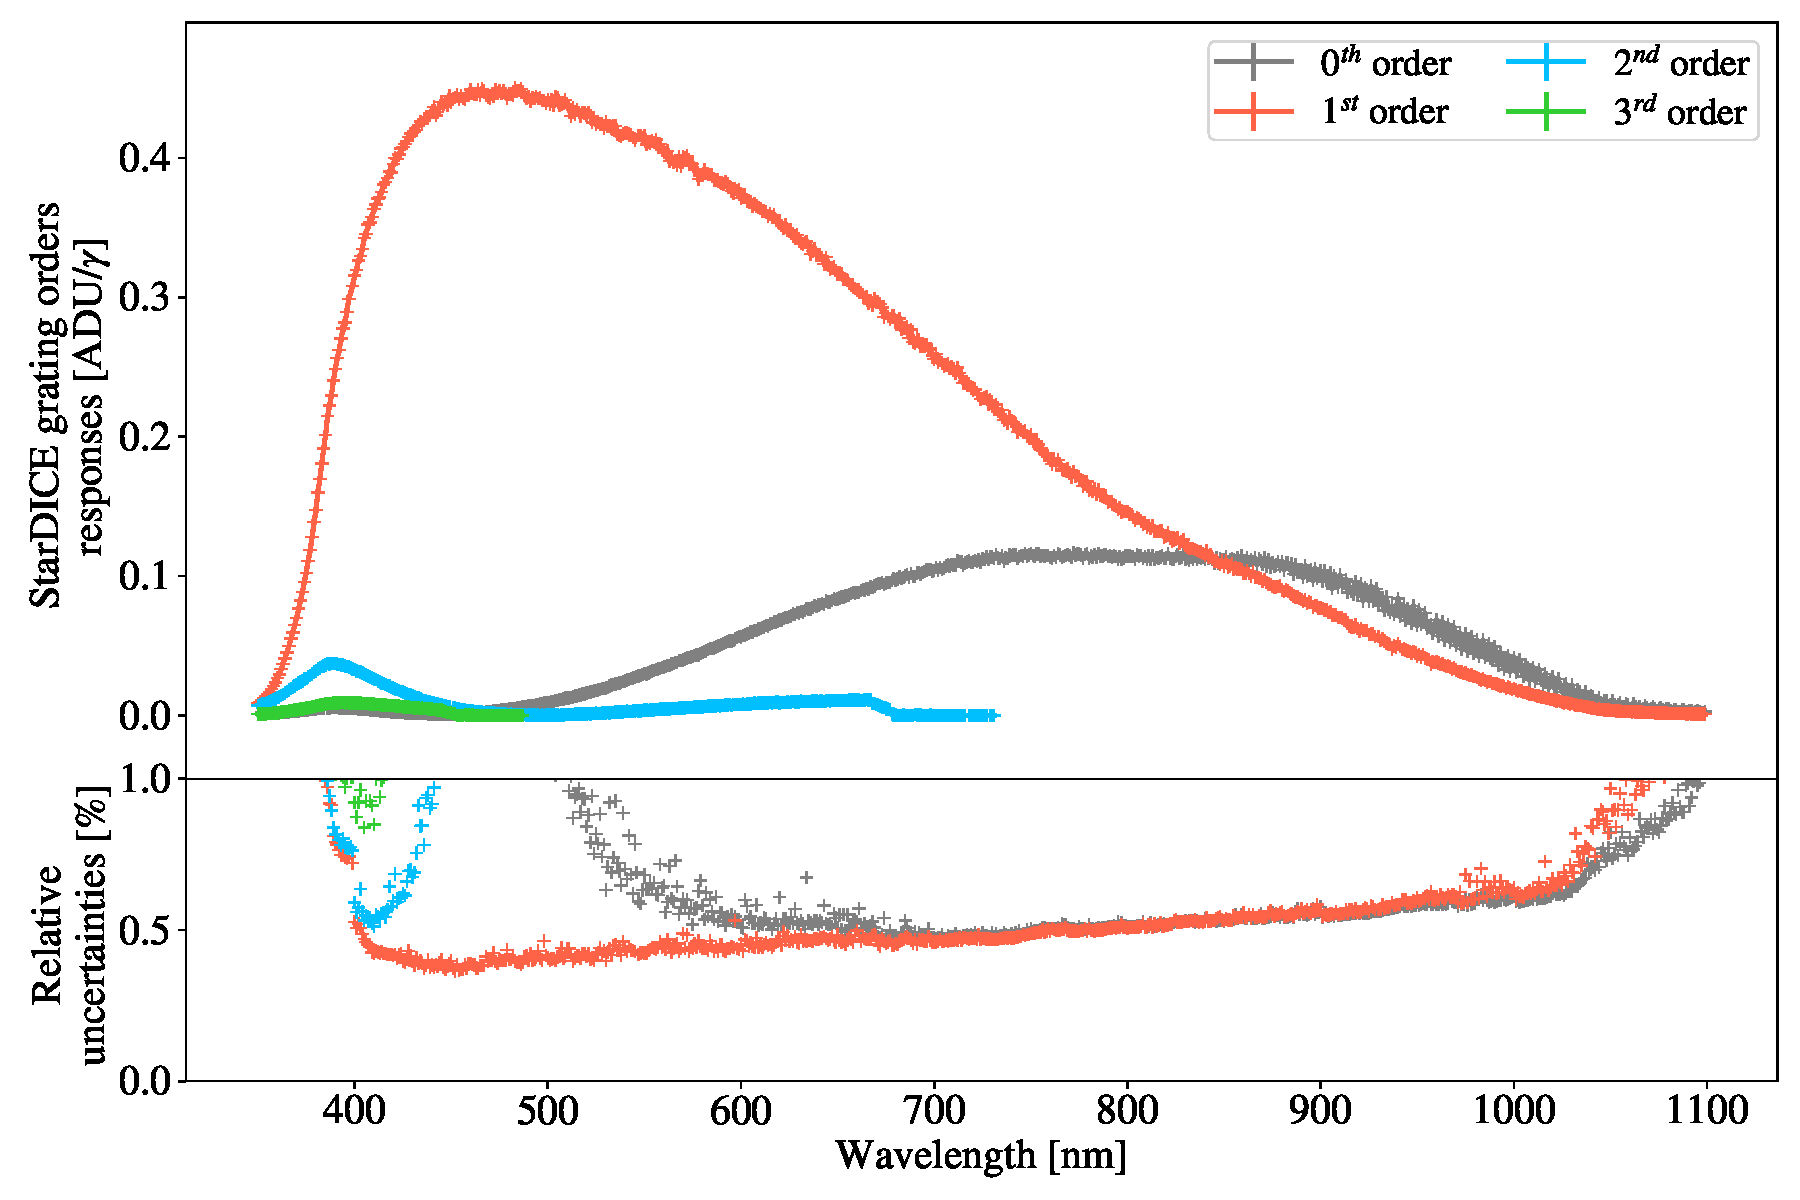
\includegraphics[width=\columnwidth]{fig/stardice_grating_response.pdf}
    \caption{Up : \SD response with the grating in front of the camera and \spinhole pinhole with respect to wavelength in nanometer. Bottom : Uncertainties over the \SD response measurement with respect to wavelength in nanometer.}
    \label{fig:stardice_grating_response}
    %~/stardice/analysis/cbp_paper/golden_sample_analysis/dr2/response_plots.ipynb
\end{figure}

\subsubsection{Radial positions}

The upper Figure~\ref{fig:radial_positions} show the \SD response obtained with the \spinhole pinhole and without filters for the different radial positions on the mirror shown in Figure~\ref{fig:8_mirror_positions} left, and the same focal plane position. The lower figure show the normalized residuals to the mean spline going through the four responses. In the ultraviolet below \SI{450}{\nm}, we can see a significant difference between the four radial positions. It goes up to 30\%, and it will be discussed in the section \ref{sec:discussion}. What we see above \SI{1000}{\nm} in the infrared is the result of the data oscillations around the spline caused by the fringing. 

\begin{figure}[h]
    \centering
    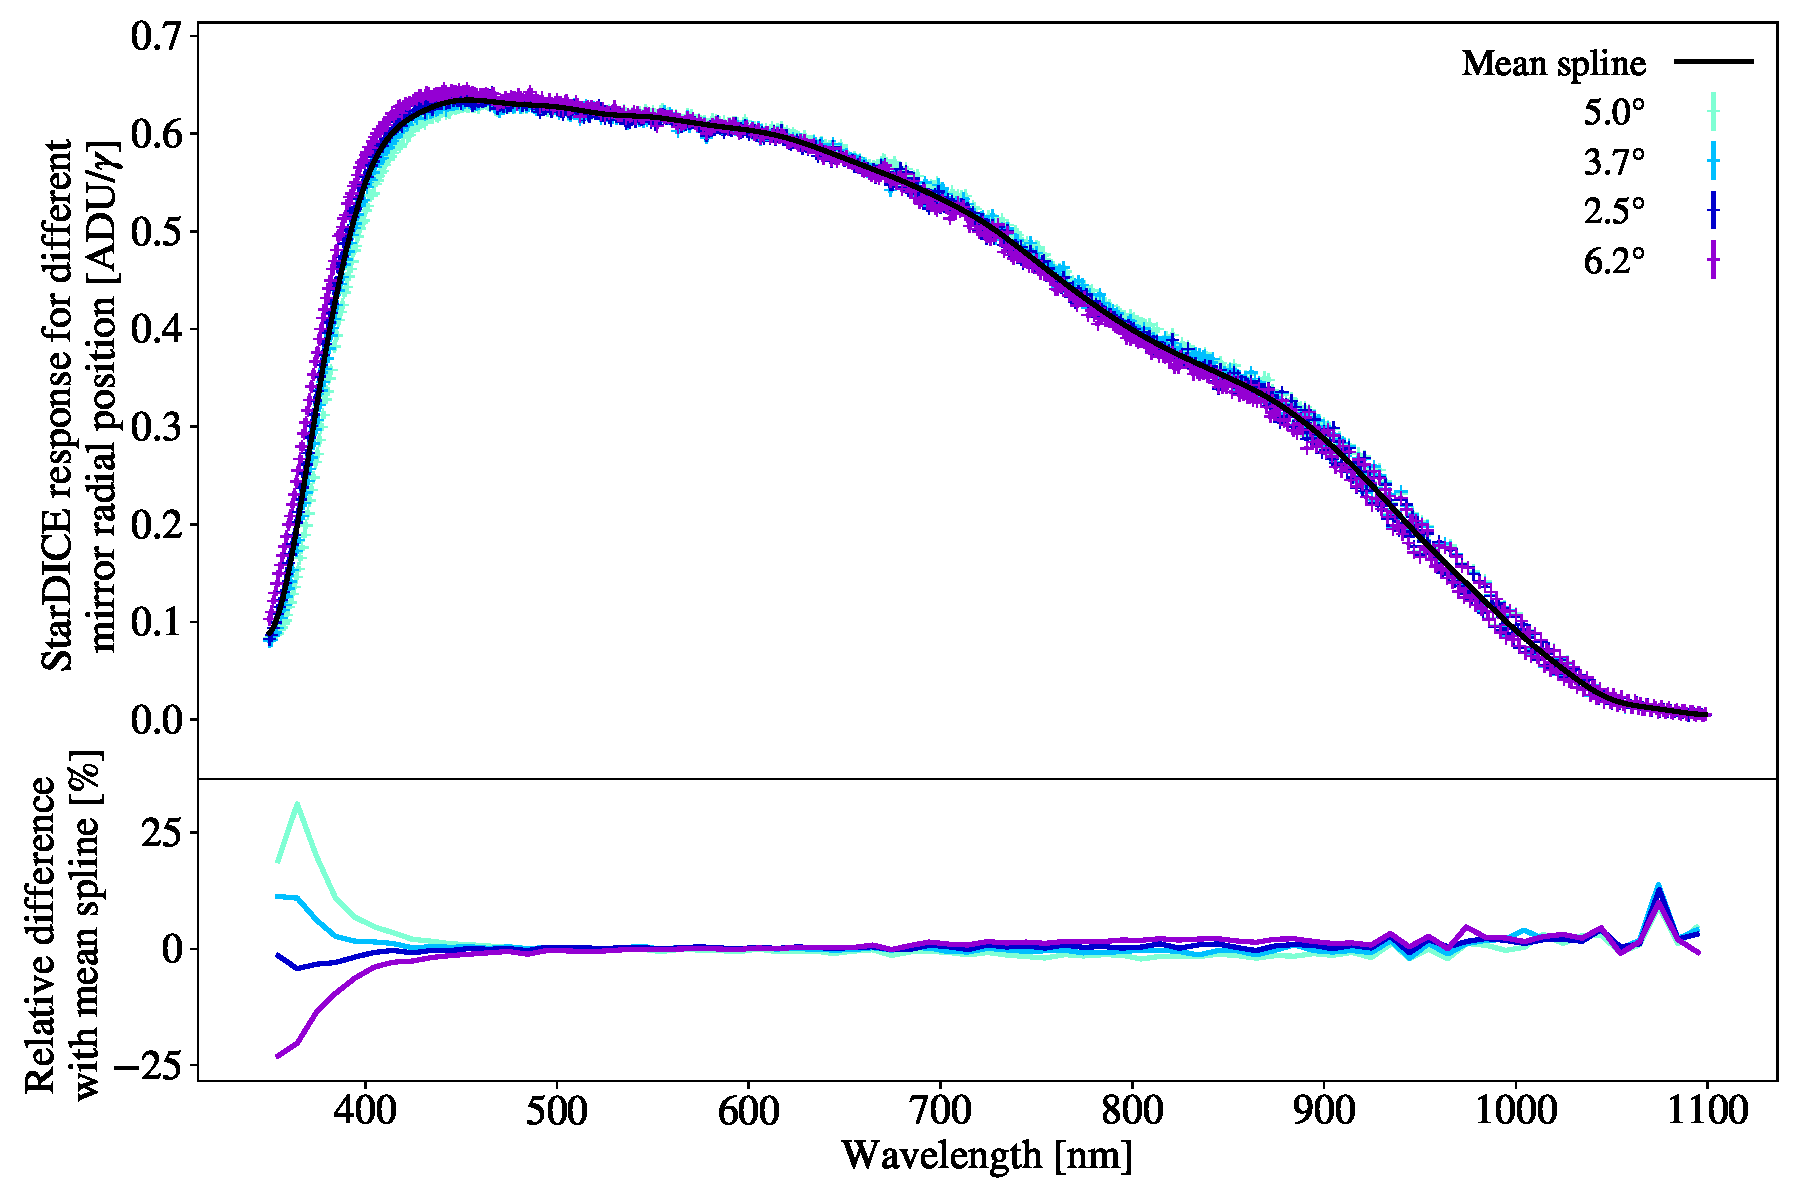
\includegraphics[width=\columnwidth]{fig/radial_positions.pdf}
    \caption{Top : \SD response for the different radial positions on the mirror, but same position on the focal plane. Bottom : Relative difference between the data and the mean spline.}
    \label{fig:radial_positions}
    %~/stardice/analysis/cbp_paper/golden_sample_analysis/dr2/2022_03_01_stardice_transmission_radius.ipynb
\end{figure}

\subsubsection{Quadrant positions}

The upper Figure~\ref{fig:radial_positions} show the \SD response obtained with the \spinhole pinhole and without filters for the different quadrant positions on the mirror shown in Figure~\ref{fig:8_mirror_positions} right, and the same focal plane position. The lower figure show the normalized residuals to the mean spline going through the four responses. We see again a divergence below \SI{400}{\nm} of about 20\% at most. The phenomenon in the infrared is still caused by the fringing. 

\begin{figure}[h]
    \centering
    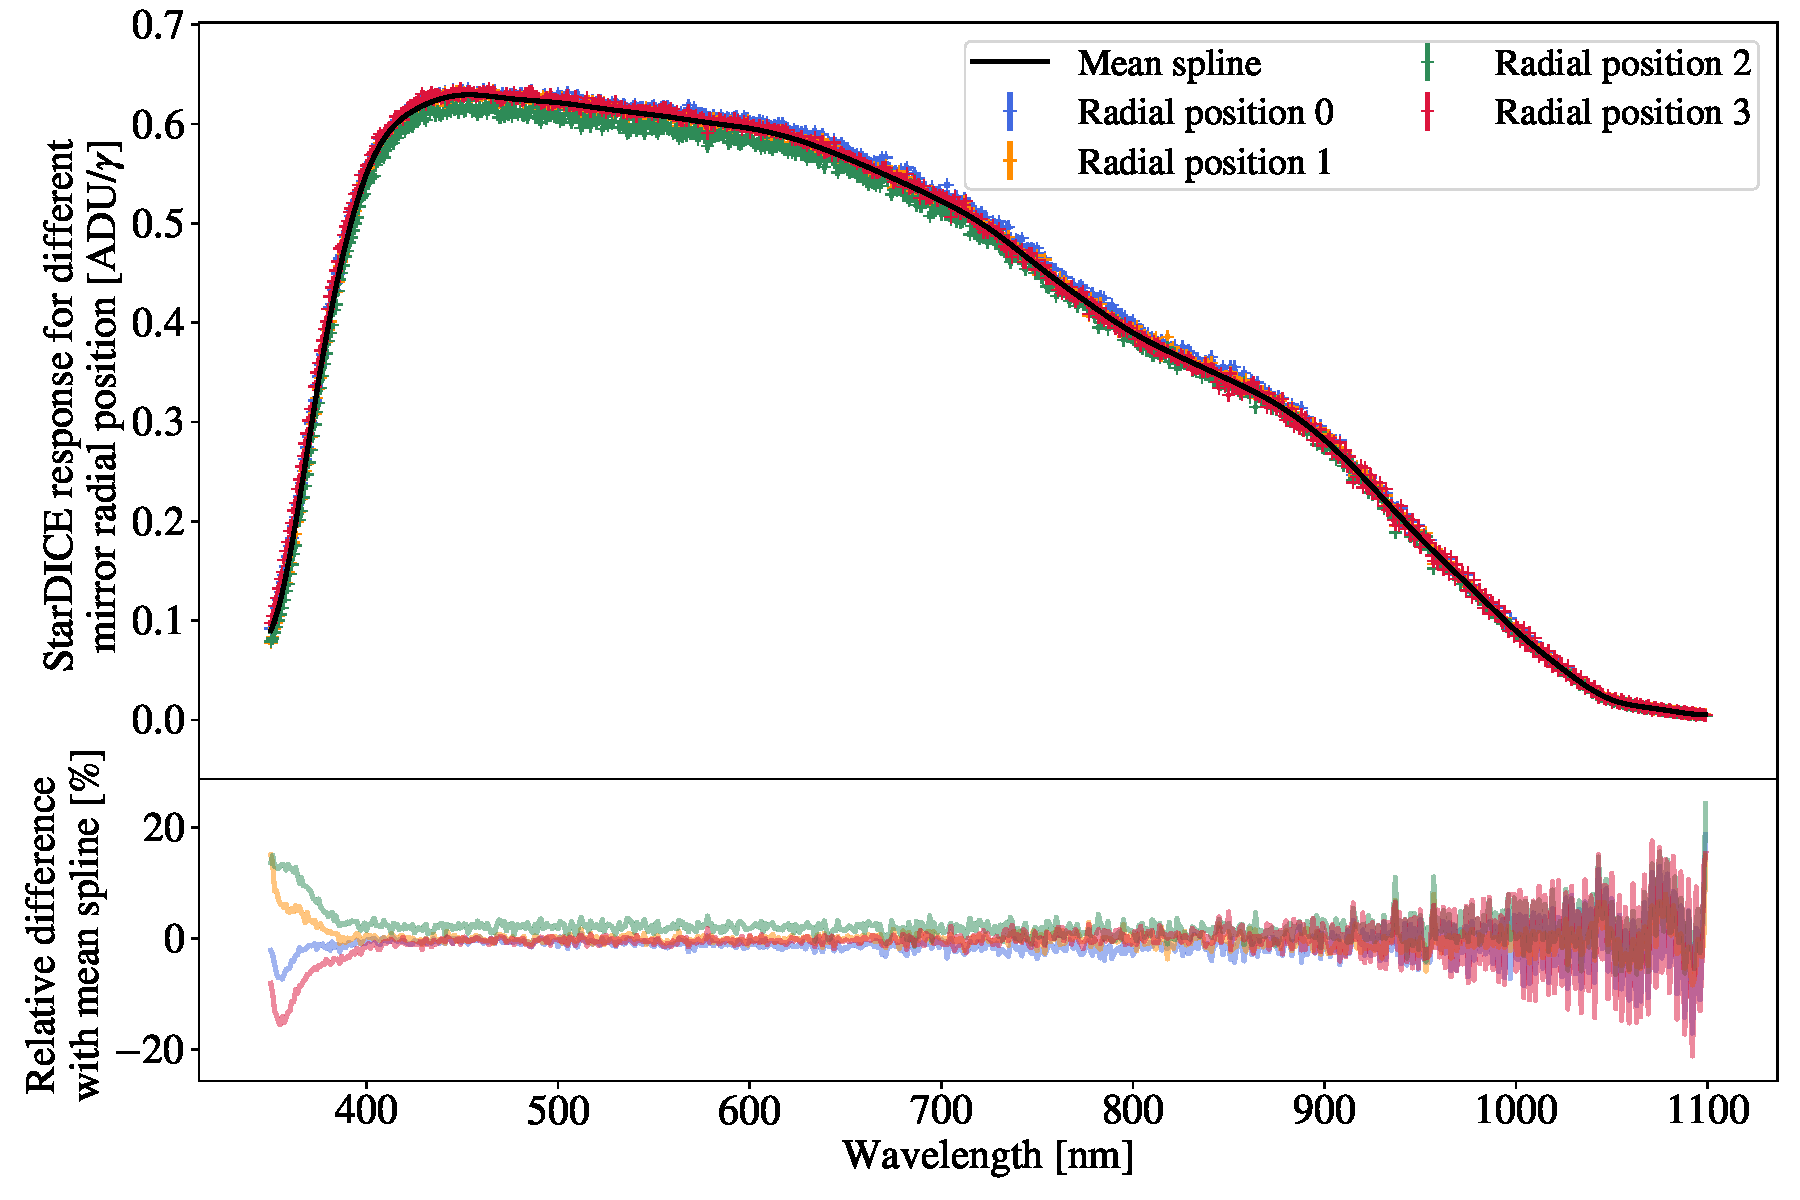
\includegraphics[width=\columnwidth]{fig/quadrant_positions.pdf}
    \caption{Top : \SD response for the different quadrant positions on the mirror, but same position on the focal plane. Bottom : Relative difference between the data and the mean spline.}
    \label{fig:quadrant_positions}
    %~/stardice/analysis/cbp_paper/golden_sample_analysis/dr2/2022_03_01_stardice_transmission_mirror_samples.ipynb
\end{figure}

\subsubsection{Focal plane positions}

The upper Figure~\ref{fig:ccd_positions} show the \SD response obtained with the \spinhole pinhole and without filters for the same radial and quadrant position on the mirror, and the different focal planes positions from the grid show in Figure~\ref{fig:ccd_grid}. The lower figure show the normalized residuals to the mean spline going through the sixteen responses.

\begin{figure}[h]
    \centering
    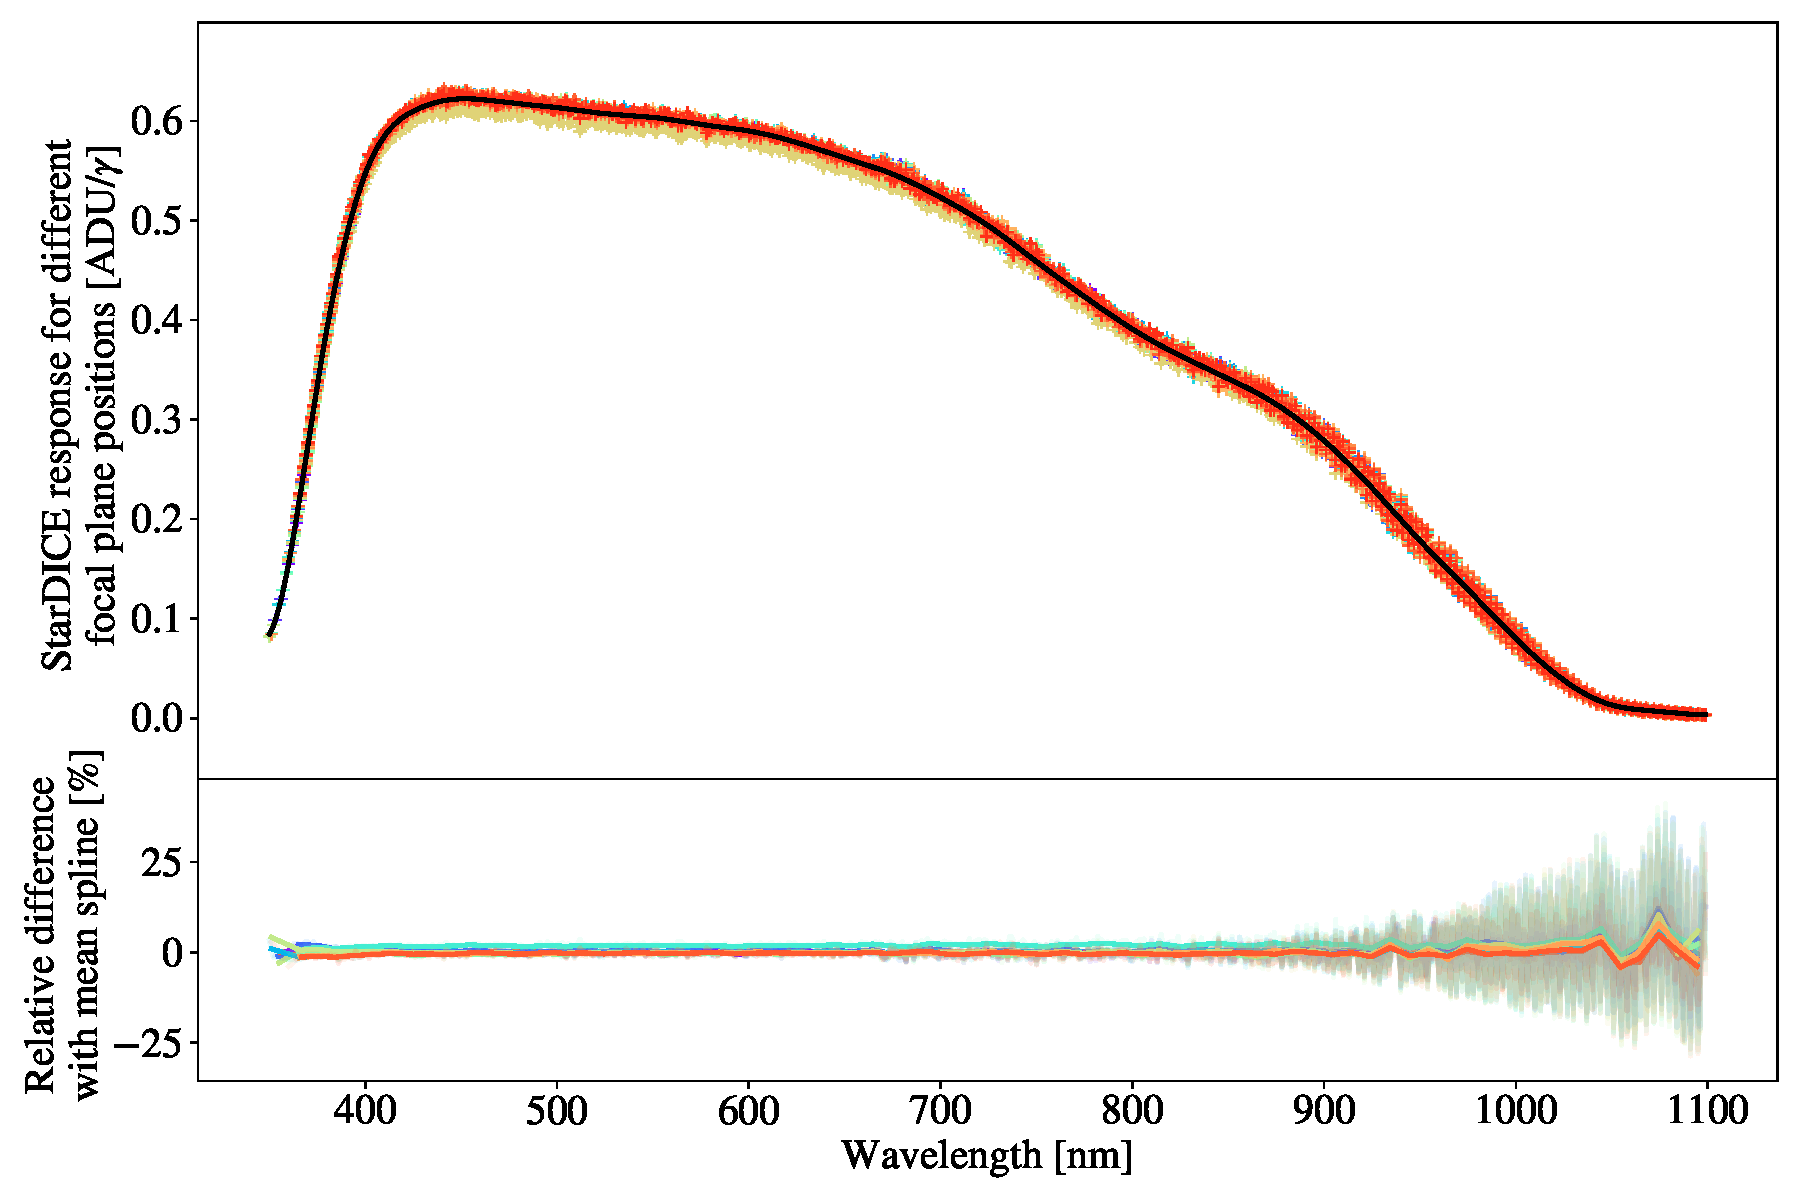
\includegraphics[width=\columnwidth]{fig/ccd_positions.pdf}
    \caption{Top : \SD response for the different positions on the focal plane, but same position on the mirror. Bottom : Relative difference between the data and the mean spline.}
    \label{fig:ccd_positions}
    %~/stardice/analysis/cbp_paper/golden_sample_analysis/dr2/2022_03_09_stardice_transmission_grid_auto.ipynb
\end{figure}

\subsection{Systematic uncertainties}
\label{sec:systematics}

\subsubsection{Stability of the StarDice responses}

\subsubsection{Gain and linearity}
\label{sec:gain}

Varying pinhole with StarDice, and CBP
Varying QSW but depending on result it falls into this subsection or the following

\subsubsection{Pinhole chromaticity}

\subsubsection{Pull distributions}

\subsubsection{Courbes de croissances}




